\documentclass{article}
% Tamaño página
\usepackage[paperheight=27cm,paperwidth=21cm,textwidth=19cm ,textheight=23cm]{geometry}
% Librería lorem ipsum?
\usepackage{lipsum}
\usepackage{fancyhdr}
\usepackage{hyperref}
\usepackage{graphicx}
\graphicspath{{images/}}
\hypersetup{
    colorlinks=true,
    linkcolor=blue,
    filecolor=magenta,      
    urlcolor=cyan,
    pdftitle={Laboratorio 3 - Switches administrables - Mariano Campos},
    pdfpagemode=FullScreen,
    }

\title{\bfseries \huge Laboratorio 3 - Switches Administrables \normalsize{\linebreak\\Redes de computadoras I \\Prof.: Walter Lozano\\Prof.: Alejandro Rodriguez Costello}}
\author{\\\\\\\\\\\\Campos, Mariano Andrés \\ {\small visual.design.90@gmail.com}}
\date{\small 11 de Septiembre 2024}

\begin{document}
    \maketitle
    \newpage

    \section{Escenario 1}
    \subsection{Spanning Tree Protocol (STP)}
    Al cargar el escenario solicitado, lo primero que se puede apreciar es que los 3 routers comienzan a autoconfigurarse (se puede apreciar un punto naranja en cada una de las conexiones físicas). Pasado algunos segundos estos puntos naranjas se transforman en un triangulo verde indicando que la conexión es correcta y se puede transmitir información entre los dispositivos exceptuando el switch1, el cual aún presenta un punto naranja en su conexión con el Switch0.

    \begin{center}
        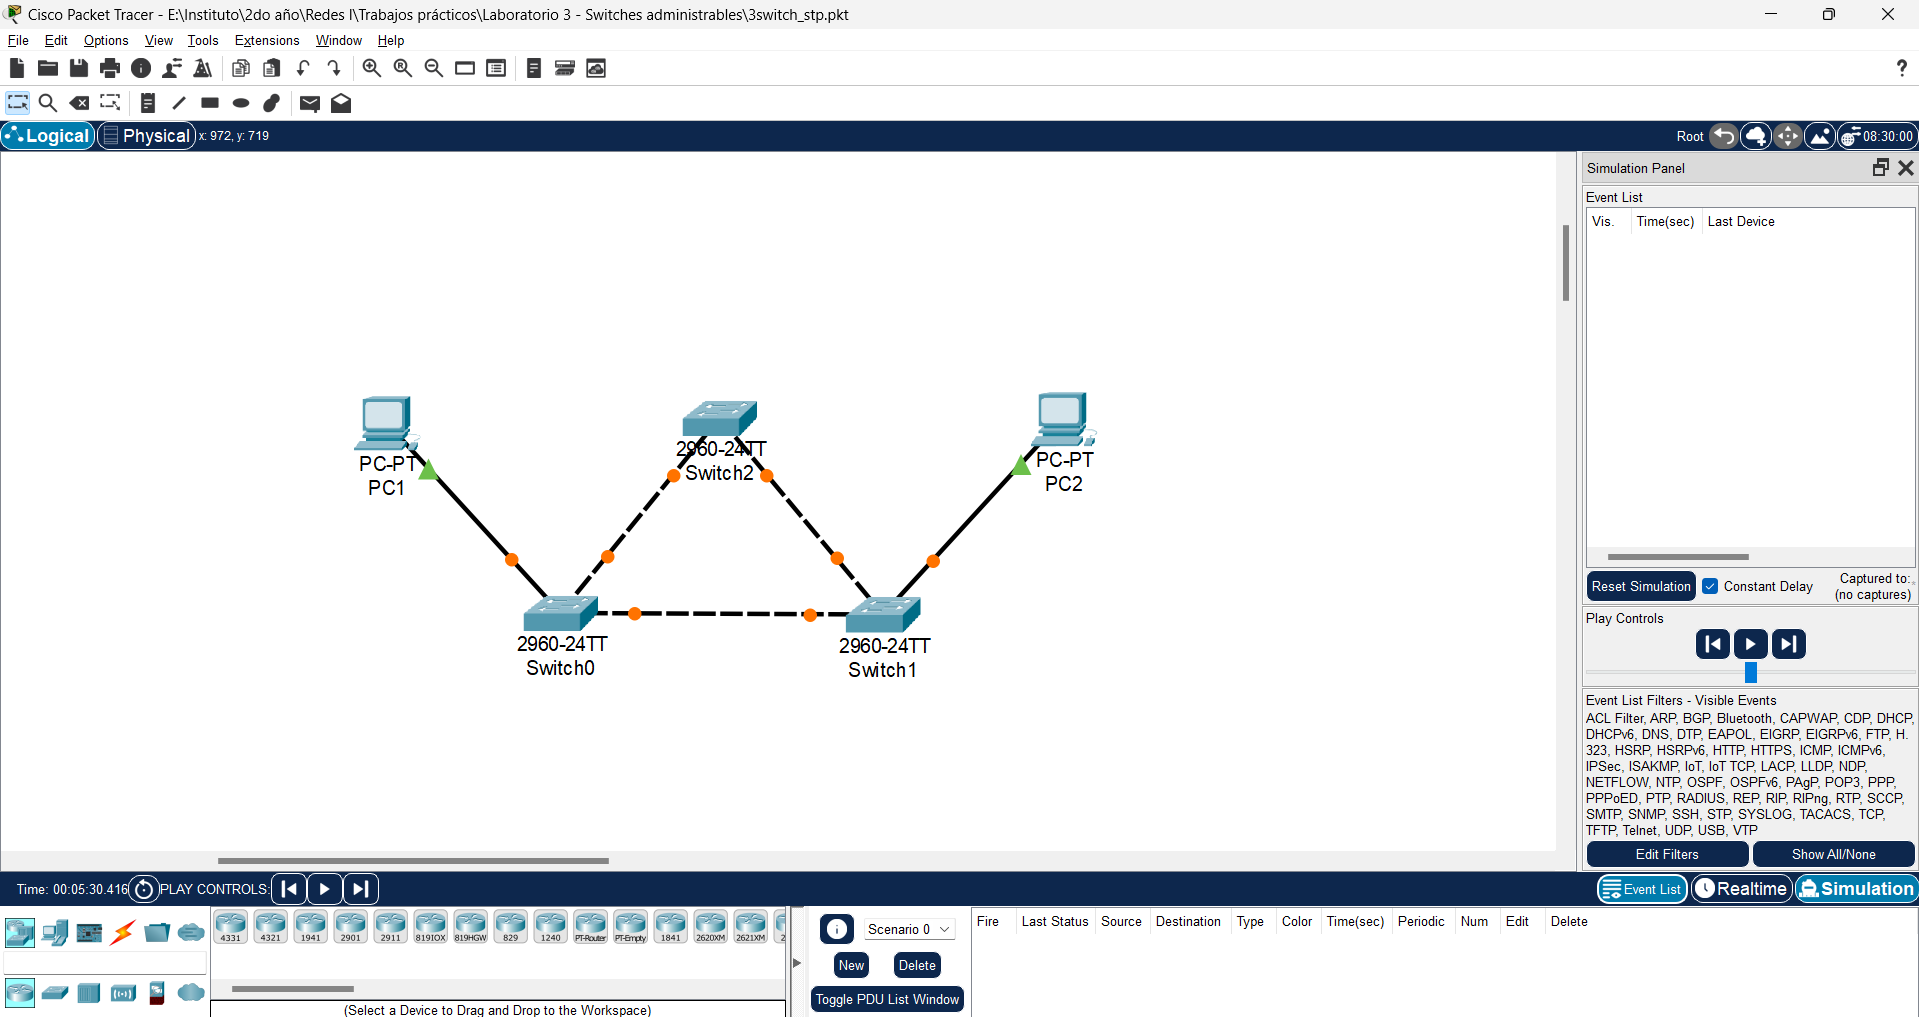
\includegraphics[width=0.475\linewidth]{img_01} 
        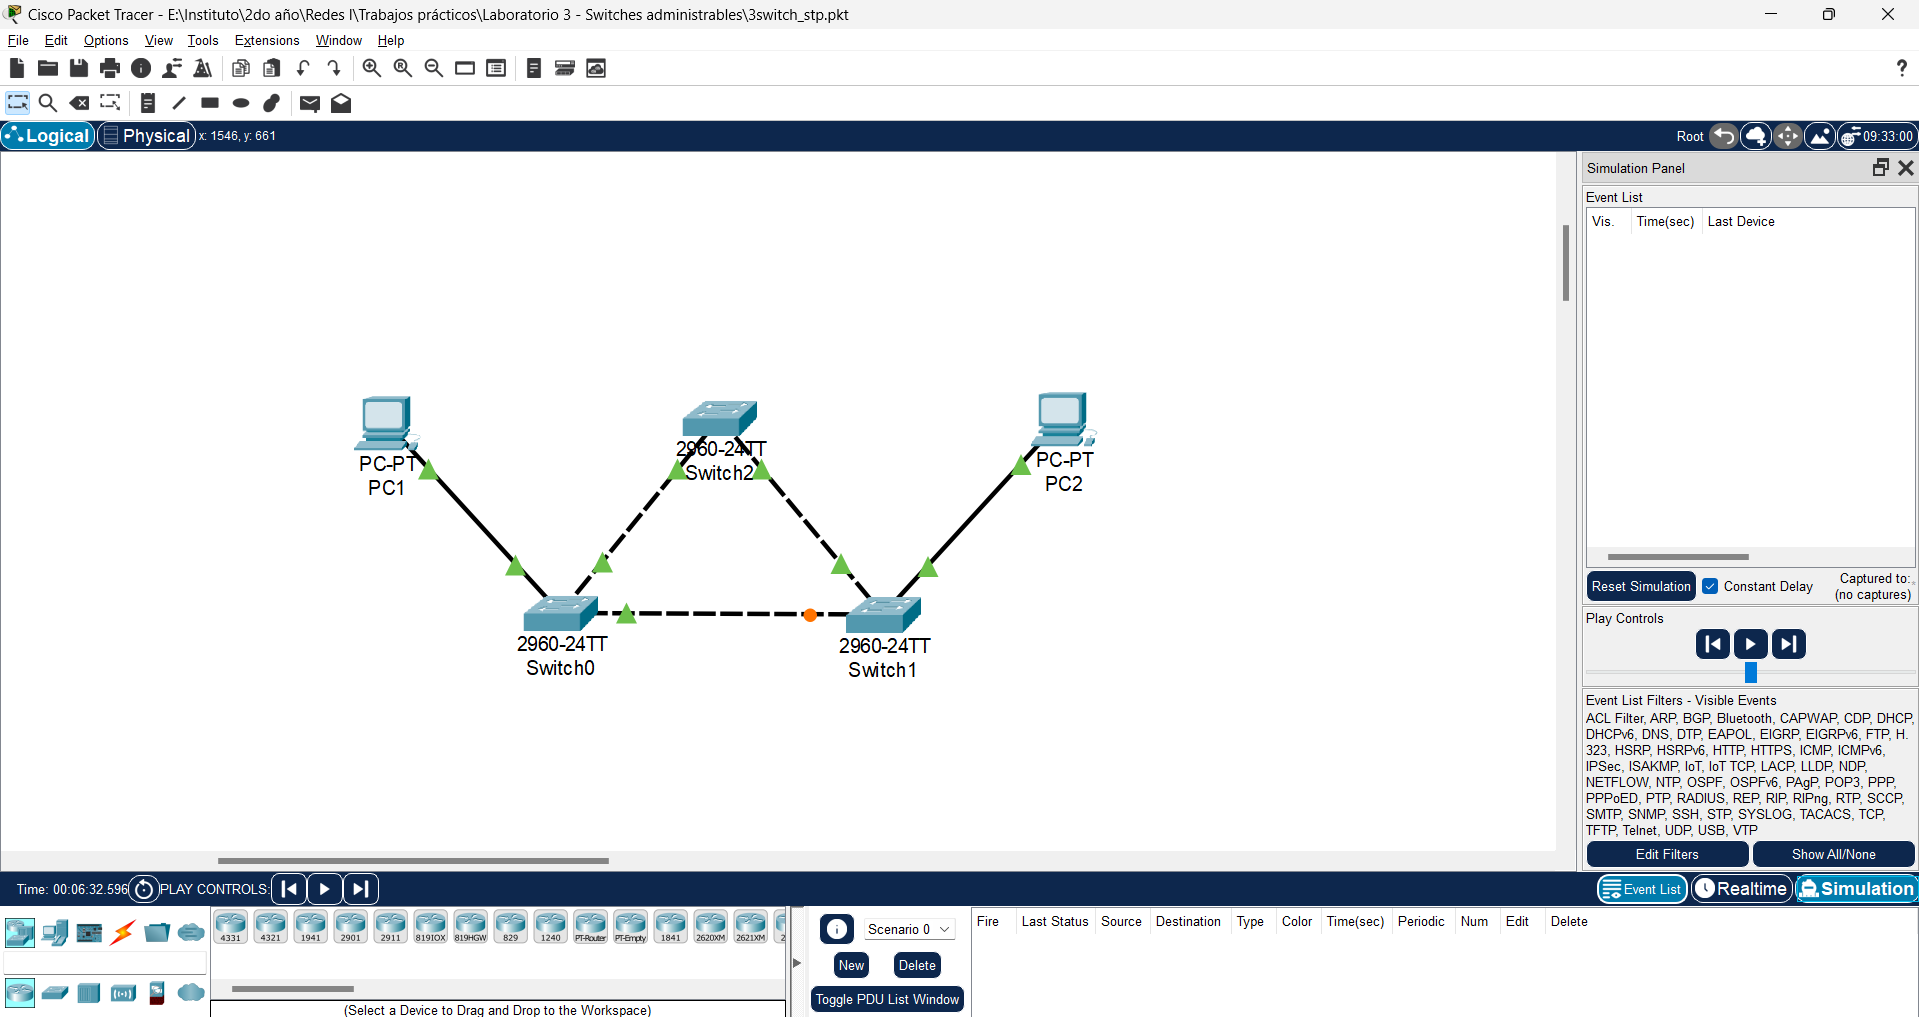
\includegraphics[width=0.475\linewidth]{img_02} 
        \linebreak
        \small {\bfseries Figura 1}: Esquema redundante de switches pre y post autoconfiguración.
    \end{center}

    Utilizando un PDU para enviar un mensaje del PC1 al PC2 lo primero que sucede es que en la PC0 se configuran 2 paquetes. El primer paquete es de tipo ARP, el cual mediante un broadcast solicitará a cada dispositivo de la red, la dirección MAC que corresponda a la pc con la que se quiere conectar, debido a que la caché ARP de PC1 se encuentra vacía. El paquete enviado viaja al Switch0, el cual se encarga de enviar el broadcast a todas sus conexiones activas. Dos paquetes ARP son enviados, uno al Switch2, y otro al Switch1 quien parece descartar este paquete.\\
    Posteriormente el Switch2 envía el ARP al Switch1 (lo recibe 2 veces) pero esta vez no lo descarta y lo envía a PC2. El paquete ARP llega correctamente viajando de PC1 → Switch0 → Switch2 → Switch0 → PC2 y de vuelta realizando el mismo camino.

    \begin{center}
        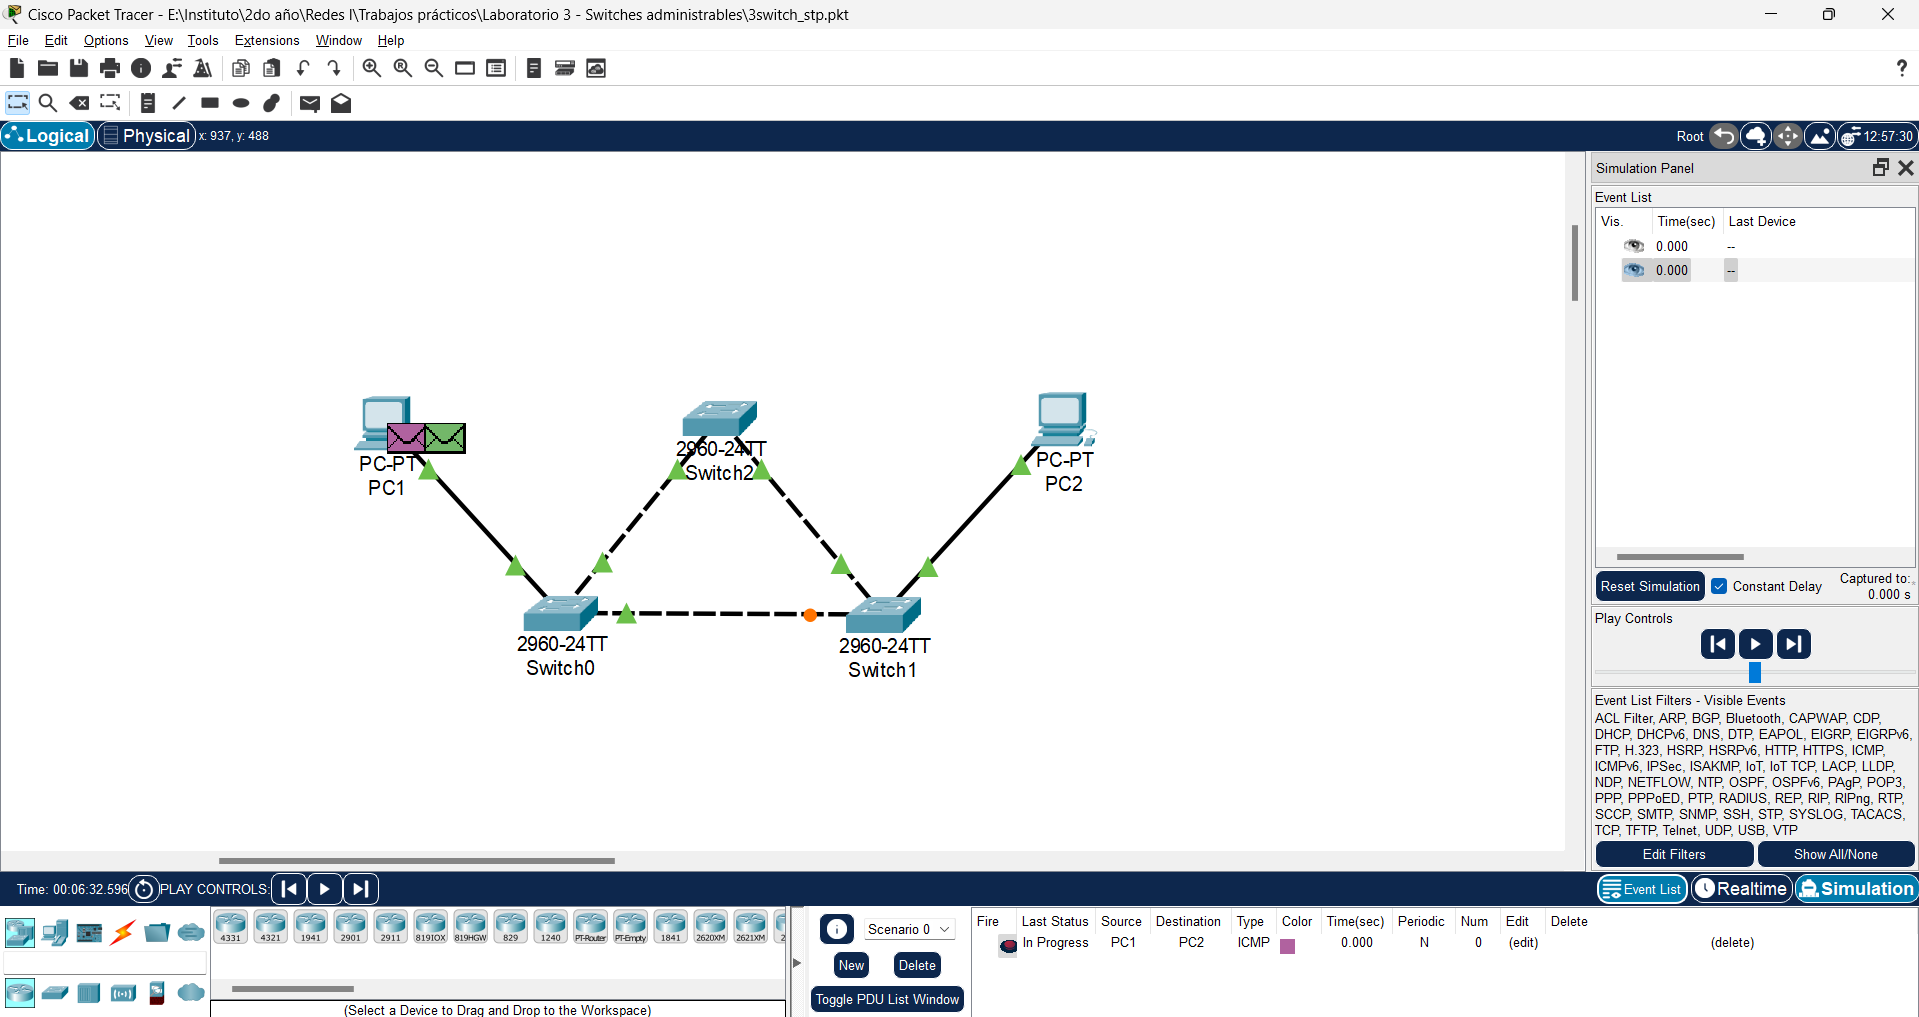
\includegraphics[width=0.875\linewidth]{img_03} 
        \linebreak
        \small {\bfseries Figura 2}: Seteo de primer comunicación entre PC1 y PC2.
    \end{center}

    \pagebreak
    El paquete ARP arriba correctamente y en este punto la PC1 puede realizar la comunicación solicitada, ya que conoce cómo comunicarse con PC2, y su caché ARP se encuentra ahora actualizada con la información de PC2. La comunicación se realiza siguiendo el camino mencionado anteriormente del PC1 al PC2.

    \begin{center}
        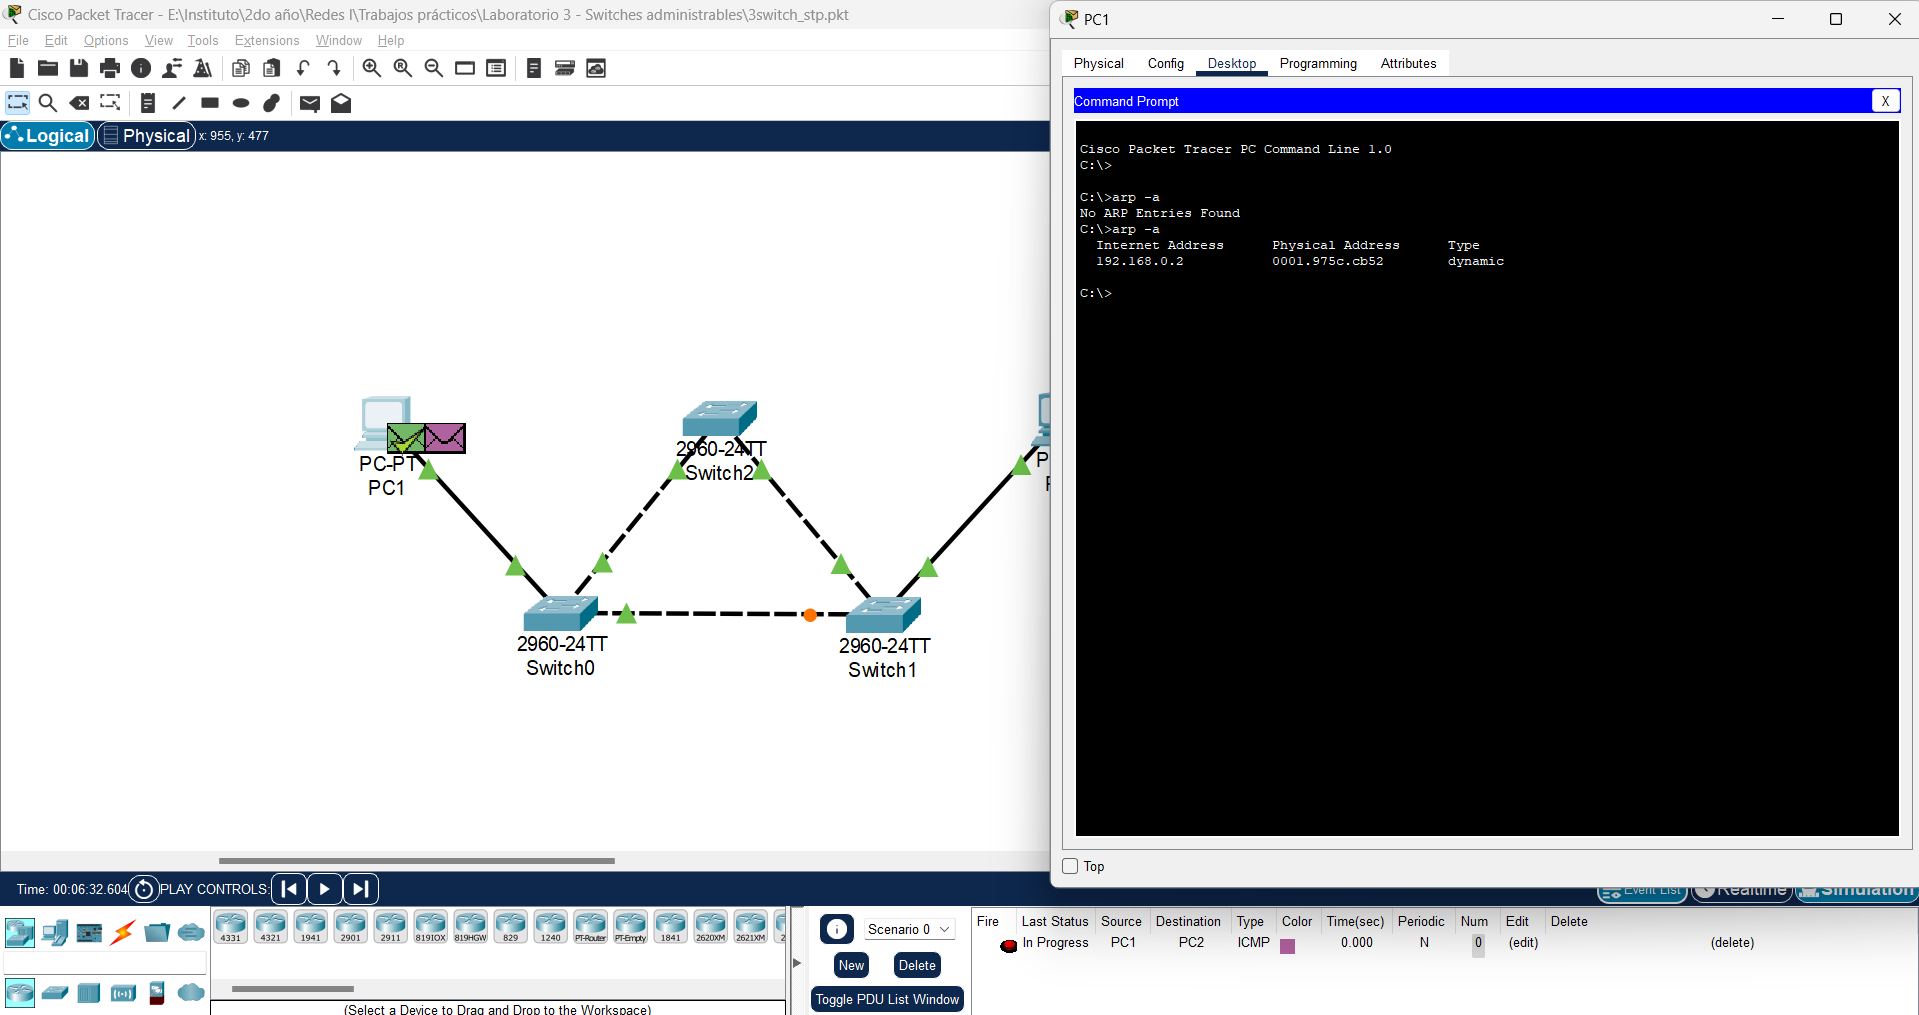
\includegraphics[width=0.875\linewidth]{img_04} 
        \linebreak
        \small {\bfseries Figura 3}: ARP correcto en PC1 y caché ARP actualizado.
    \end{center}

    Información recopilada de los routers con comando {\bfseries show spanning-tree vlan 1}:

    \begin{center}
        \begin{tabular}{| p{3cm} | p{4.1cm} | p{4.1cm} | p{4.1cm} |}\hline
            {\bfseries Dispositivo} & {\bfseries Address} & {\bfseries Bridge ID Priority} \\\hline
            Switch0 & 0001.C7E4.67A1 & 32769 \\\hline
            Switch1 & 0090.2B6C.AD29 & 32769 \\\hline
            Switch2 & 0001.C7E4.67A1 & 32769 \\\hline
        \end{tabular}
    \end{center}

    En el {\bfseries Switch0} todas las interfaces tienen estatus FWD lo que indica que tienen habilitada la comunicación. Adicionalmente la interfaz Fa0/1 tiene el rol ROOT, mientras que las otras interfaces (Fa0/2 y Fa0/3) presentan rol Desg.\\
    En el {\bfseries Switch1} la interfaz Fa0/1 tiene estatus BLK, entonces se encuentra bloqueada por el protocolo STP para evitar bucles de red. Adicionalmente las interfaces Fa0/2 y Fa0/3 tienen estatus FWD. También podemos observar en este switch que la interfaz Fa0/2 tiene rol Root (que se conecta al switch raíz), la interfaz Fa0/3 tiene rol Desg (que es la elegida para transmitir el tráfico de red) y por último la interfaz bloqueada Fa0/1 tiene rol Altn (que indica que esta interfaz es alternativa, y será utilizada en caso de que la interfaz principal (desg) falle).\\
    Por último, el {\bfseries Switch2} todas las interfaces tienen estatus FWD y rol Desg.

    \begin{center}
        \begin{tabular}{| p{2cm} | p{3.1cm} | p{2.1cm} | p{2.5cm} | p{2.5cm} | p{2.5cm} |}\hline
            {\bfseries Disp.} & {\bfseries Address} & {\bfseries BID Pty.} & {\bfseries Fa0/1} & {\bfseries Fa0/2} & {\bfseries Fa0/3} \\\hline
            Switch0 & 000A.F30D.B9EE & 32769 & 
            Role: Root \linebreak
            Status: FWD & 
            Role: Desg \linebreak
            Status: FWD & 
            Role: Desg \linebreak
            Status: FWD \\\hline
            Switch1 & 0090.2B6C.AD29 & 32769 & 
            Role: Altn \linebreak
            Status: BLK & 
            Role: Root \linebreak
            Status: FWD & 
            Role: Desg \linebreak
            Status: FWD \\\hline
            Switch2 & 0001.C7E4.67A1 & 32769 & 
            Role: Desg \linebreak
            Status: FWD & 
            Role: Desg \linebreak
            Status: FWD & 
            Role: - \linebreak
            Status: - \\\hline
        \end{tabular}
    \end{center}

    \pagebreak

    El switch elegido como {\bfseries root} es el Switch2, entiendo que debido a que tienen el mismo BID priority (32769) el siguiente valor que se toma en cuenta es el menor Adress, y el que tiene menor adress es el Switch2 en esta simulación. Para corroborar esto, realicé un duplicado del escenario de pruebas y reconecté los cables a fin de chequear si tenía algo que ver cómo estaban conectados los dispositivos y realicé la prueba de mensaje entre PC1(1) a PC2(1). En esta oportunidad el Switch1(1) fué el elegido como root.\\
    Realicé la prueba una vez más, esta vez sin cambiar el cableado, y allí pude ver que se eligió como root al Switch0(1)(1). En estas dos pruebas ambos switches tenían el menor valor de adress.

    \begin{center}
        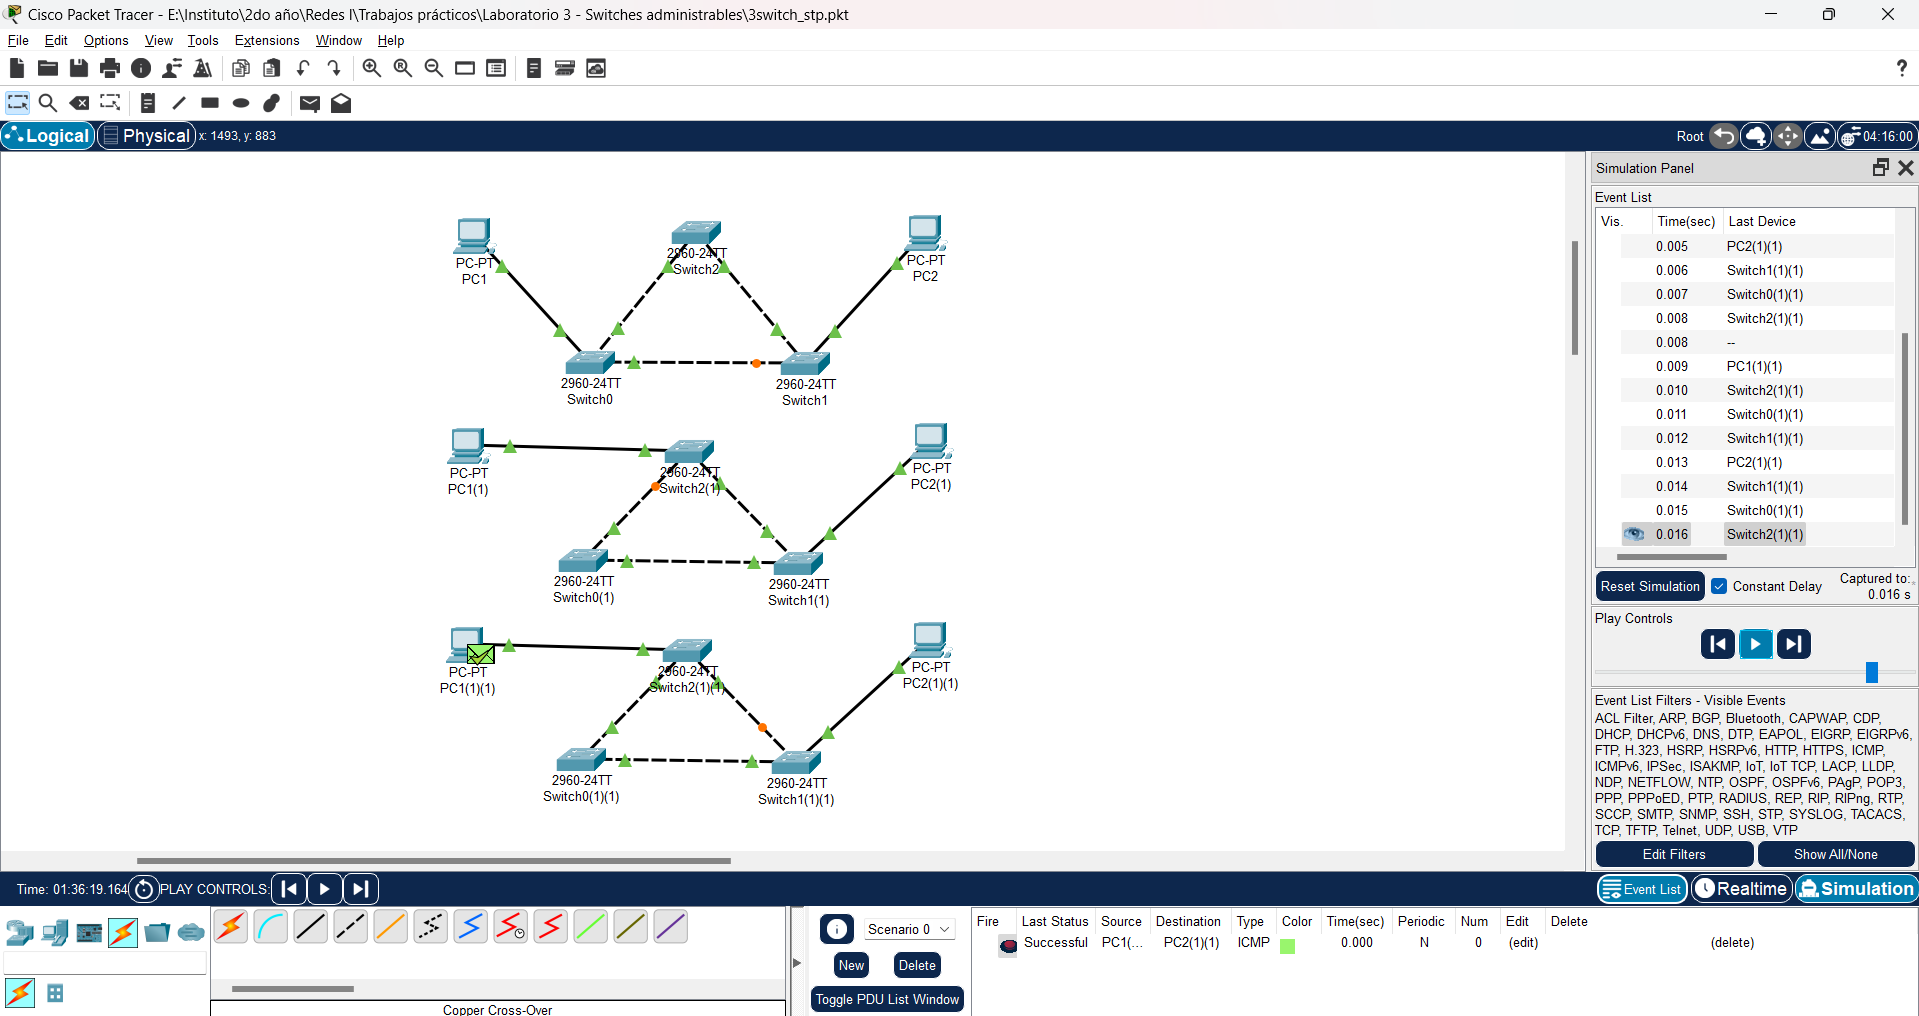
\includegraphics[width=0.875\linewidth]{img_05} 
        \linebreak
        \small {\bfseries Figura 4}: Pruebas de selección de switch root.
    \end{center}

    {\bfseries Anotaciones de comandos para las siguientes pruebas}:
    \begin{itemize}
        \item {\bfseries enable}: habilita privilegios del nivel ejecutivo, puede pedir contraseña si está configurada y se indica con el símbolo "\#". Se deshabilita con el comando disable. Ej.: \\
        Switch$>$ enable \\
        Switch\# disable \\
        Switch$>$ |
        \item {\bfseries configure terminal (conf t)}: permite acceder al modo de configuración global, se activa posterior al comando enable. Se puede configurar interfaces, vlan, ip address, routing, spanning-tree. Se sale de este modo mendiante end o exit o CTRL+Z. Ej.: \\
        Switch$>$ enable \\
        Switch\# conf t \\
        Switch(config)\# exit \\
        Switch\# disable \\
        Switch$>$ |
        \item {\bfseries interface}: este comando permite configurar las interfaces de un switch, por ejemplo activandola o desactivandola. Sólo se puede activar en modo configuración de terminal. Ej.: \\
        Switch(config)\# interface fastEthernet 0/2 \\
        Switch(config-if)\# shutdown (cambia estado a down (apagado)) \\
        Switch(config-if)\# no shutdown (cambia estado a up)
    \end{itemize}

    \pagebreak

    Al apagar la interfaz 0/2 del Switch2 se cancela la comunicación directa con el Switch1 y al Switch1 se le desbloquea la conexión con el Switch0 debido a que no habría redundancia en la red. El Switch2 continúa siendo root. \\
    Con la caché ARP de la PC1 con los datos de la PC2, realicé un envío de paquete de PC1 a PC2 con esta configuración y el paquete viajó correctamente de PC1 al Switch0, el Switch0 envió el paquete a Switch2 (quien no lo descartó) y a Switch1, que posteriormente lo entregó a su destinatario la PC2.
    
    \begin{center}
        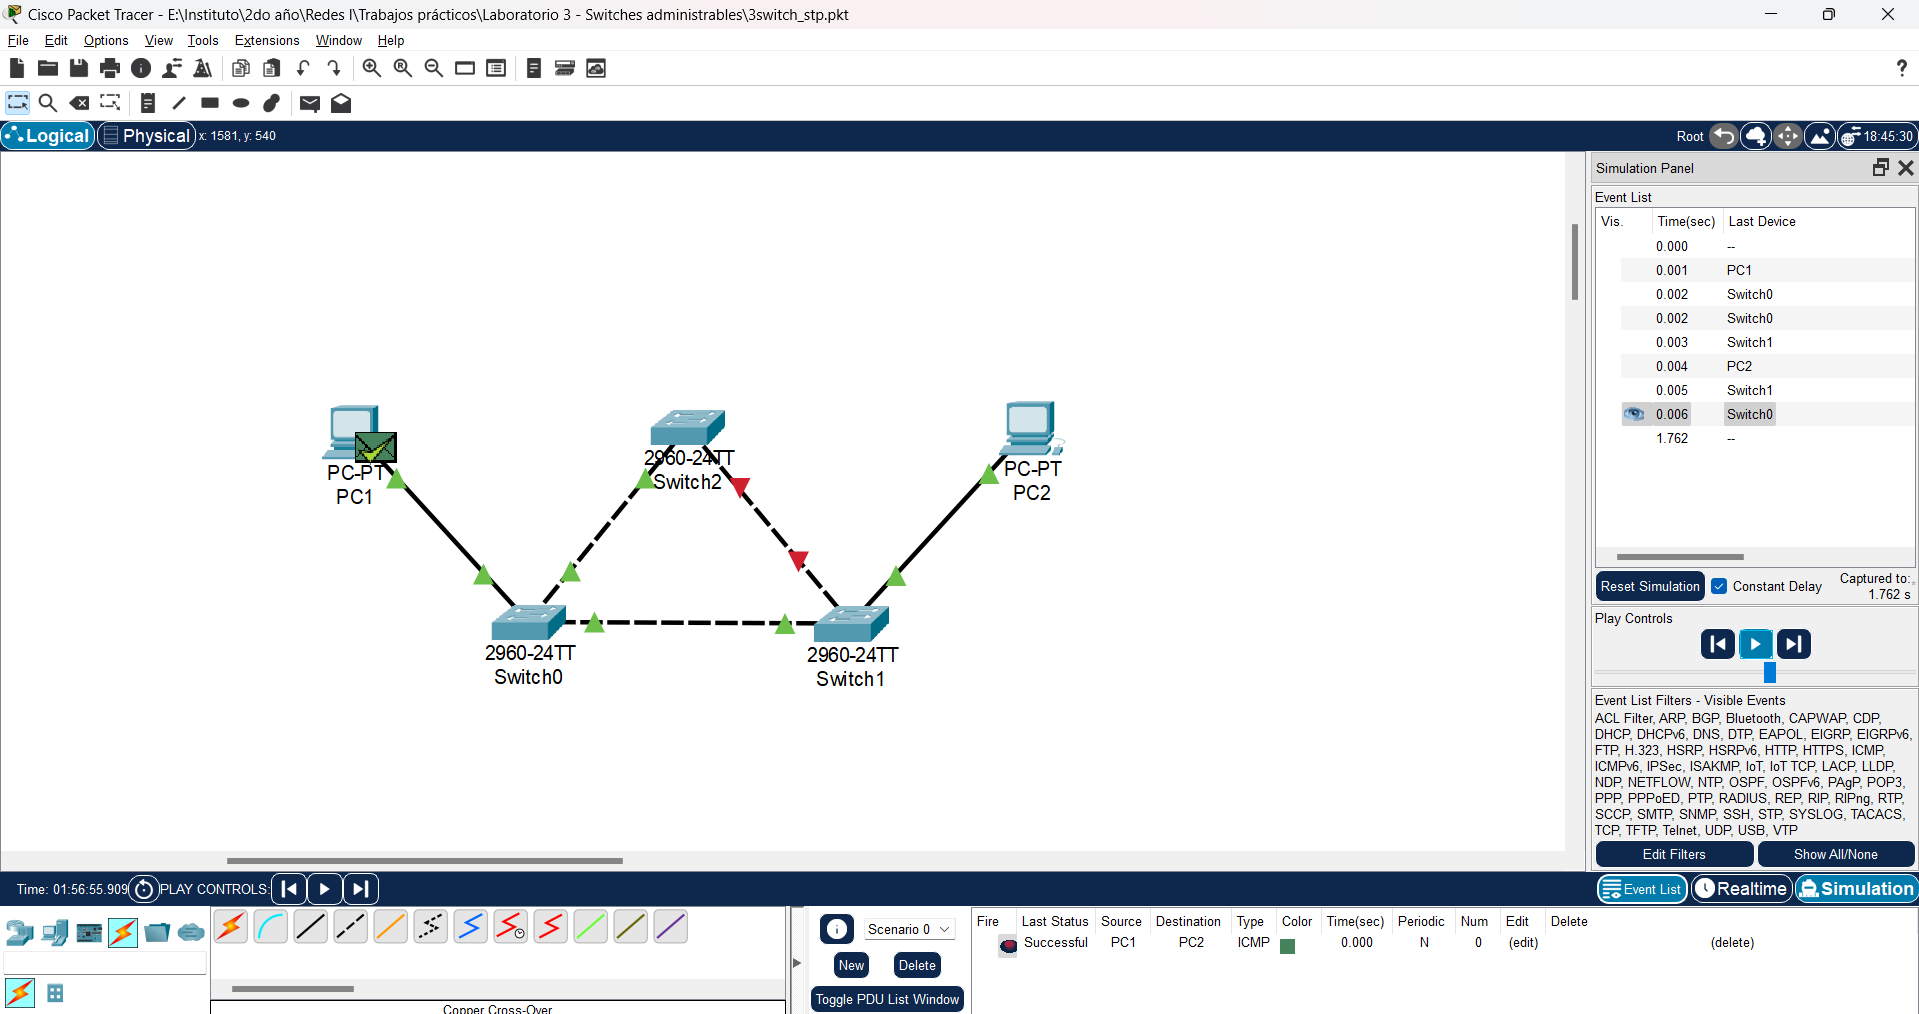
\includegraphics[width=0.875\linewidth]{img_06} 
        \linebreak
        \small {\bfseries Figura 5}: Mensaje PC1 a PC2, interfaz 0/2 del Switch1 apagada, se mantiene root y tabla ARP PC1.
    \end{center}
    
    En la figura 6 se puede apreciar de qué manera reacciona la red al limpiar la ARP de PC1, todo funciona correctamente.

    \begin{center}
        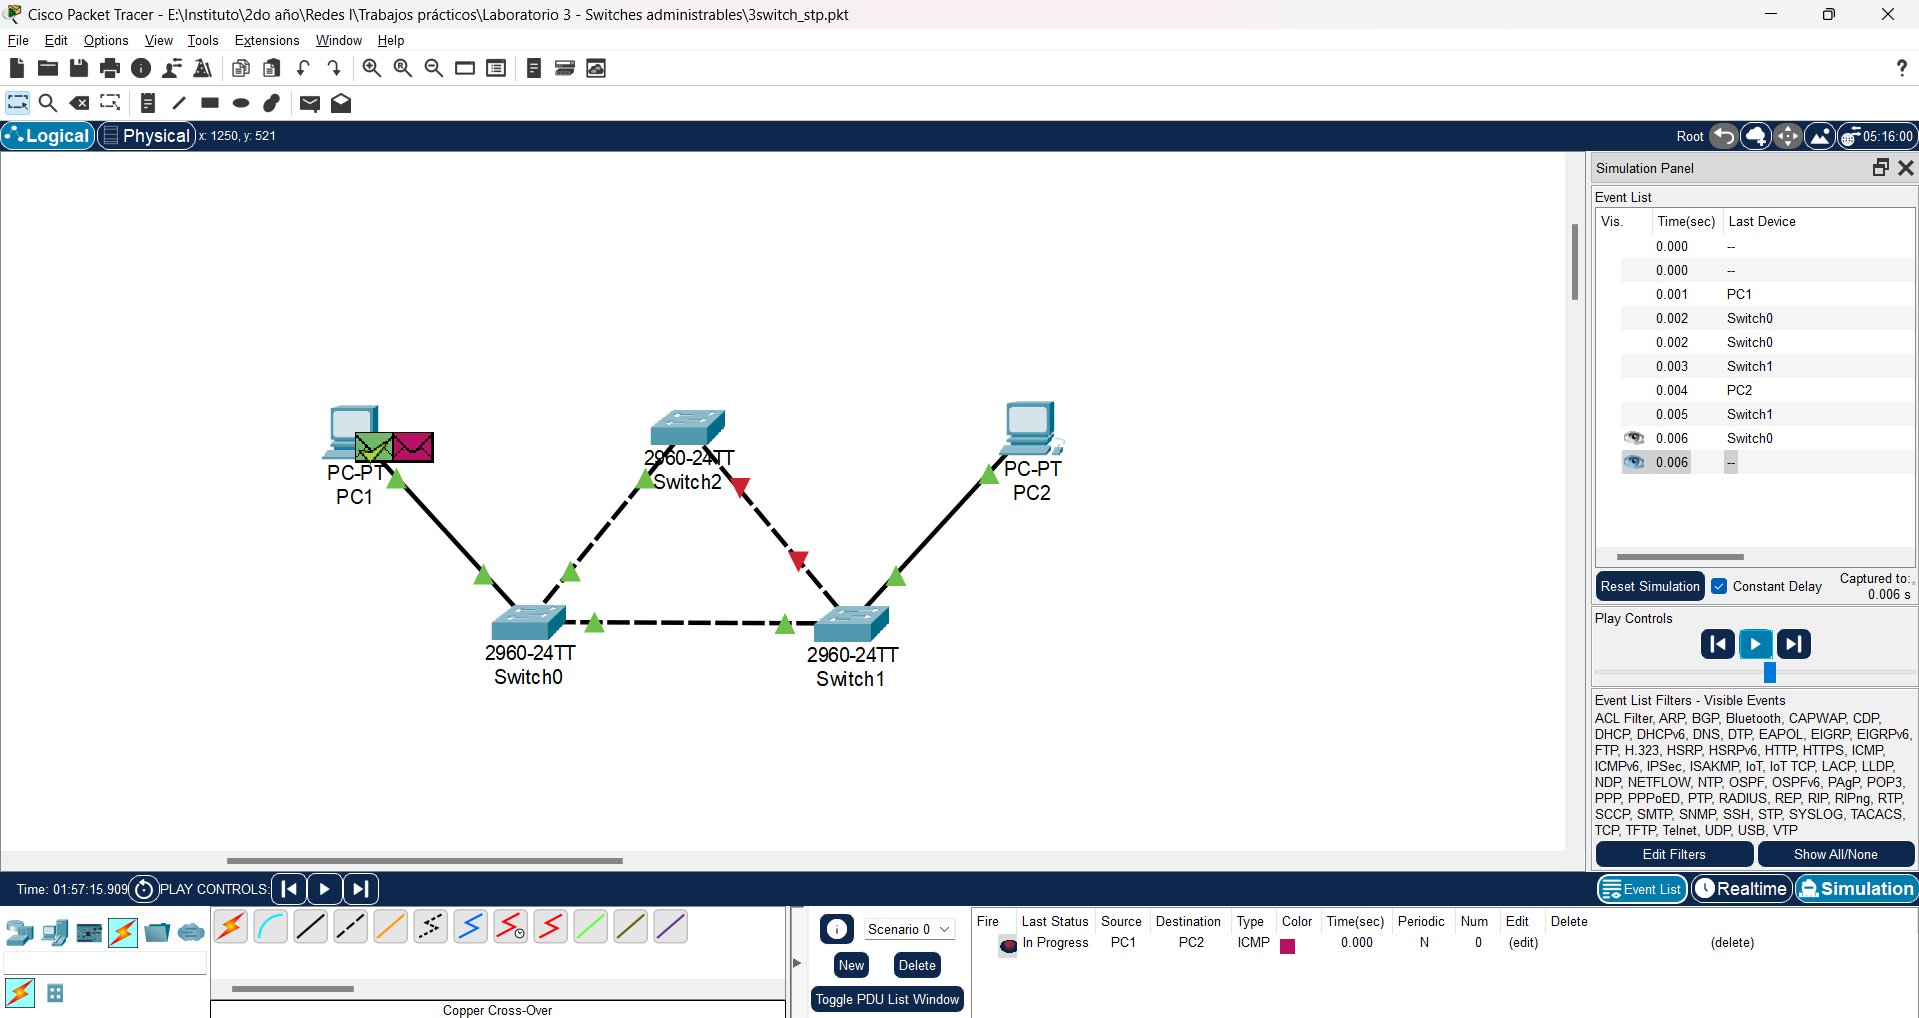
\includegraphics[width=0.875\linewidth]{img_07} 
        \linebreak
        \small {\bfseries Figura 6}: Mensaje PC1 a PC2, interfaz 0/2 del Switch1 apagada, se mantiene root y tabla ARP PC1 limpiada.
    \end{center}

    \pagebreak

    Al apagar ambas interfaces del Switch2, el siguiente switch toma su lugar como root, en este caso Switch0 (debido a que tiene el siguiente menor address).

    \begin{center}
        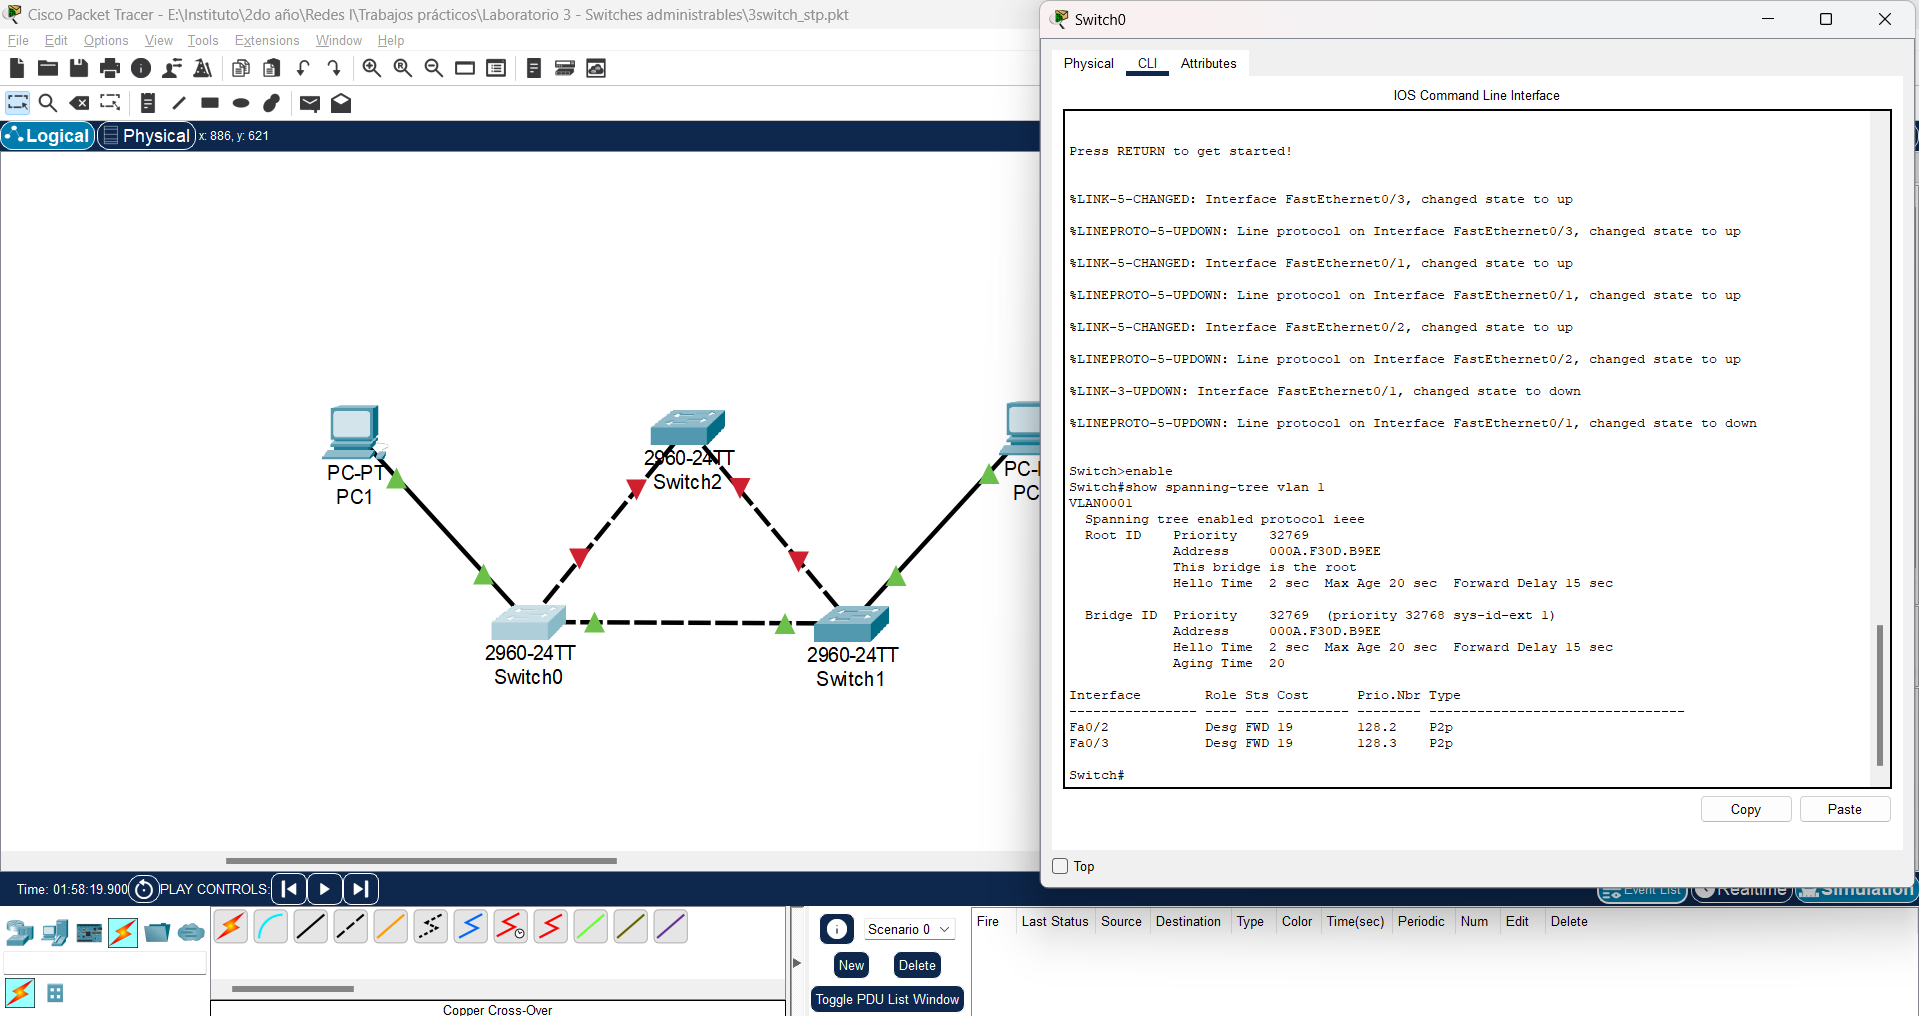
\includegraphics[width=0.875\linewidth]{img_08} 
        \linebreak
        \small {\bfseries Figura 7}: Estado de red y nuevo root.
    \end{center}

    Con el comando {\bfseries spanning-tree vlan 1 priority 57344} en el Switch0, se fuerza que el Switch1 sea el root, debido a su priority (32768+1) tiene el valor más pequeño. Esta actualización de root no se realizó hasta que corté la conexión entre ambos switches a modo de "reiniciar" las configuraciones.\\
    Entonces podemos deducir que hasta este punto, los switches cisco al tomar decisión sobre quien será root tomarán como primer valor el priority, y si este fuese igual en todos, el segundo valor a comprobar es su address (tal como se menciona en las pruebas realizadas en la figura 4).

    \begin{center}
        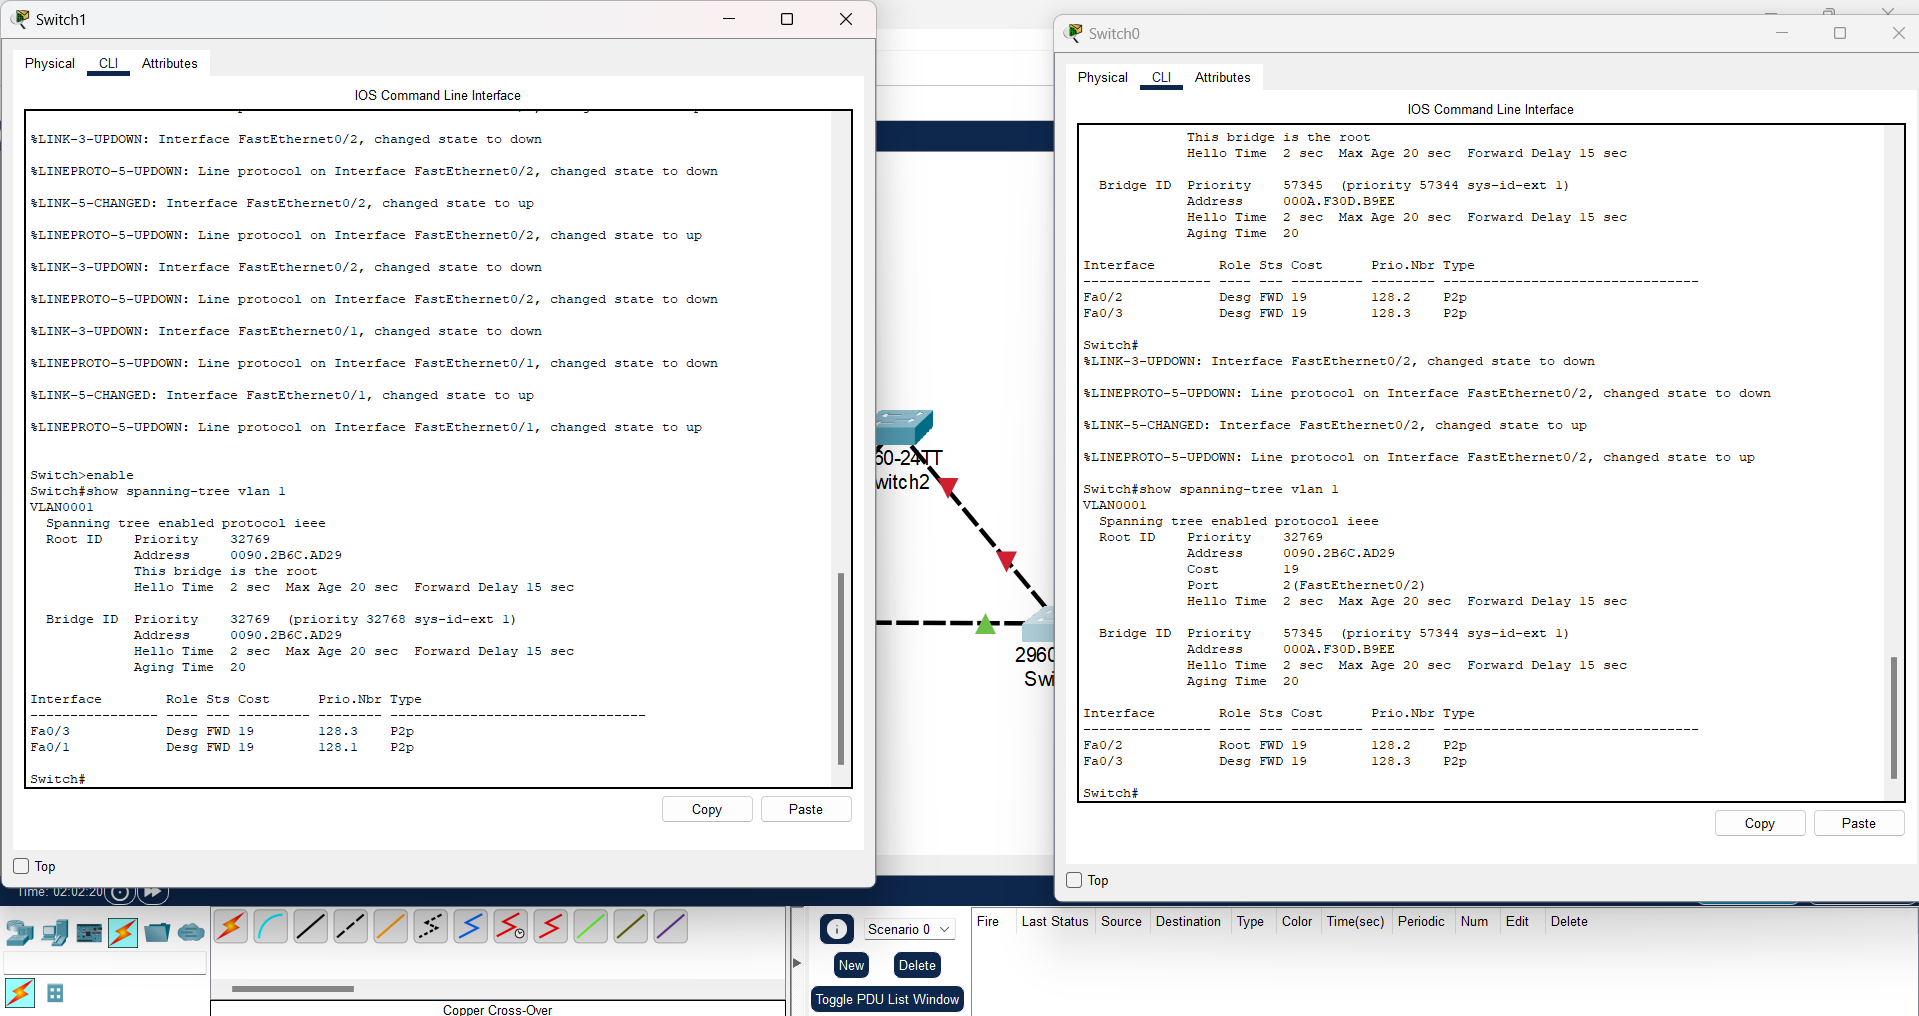
\includegraphics[width=0.825\linewidth]{img_09} 
        \linebreak
        \small {\bfseries Figura 8}: Forzado de elección root (Switch1) desde Switch0.
    \end{center}

    \pagebreak

    Al contrario de lo hecho en la figura 8, puedo setear un valor más pequeño para el Switch0 y forzar que éste sea root a pesar de tener el address mas alto.\\
    Al resetear el escenario, se puede apreciar en el CLI de Switch2 el primer comando show spanning-tree muestra que es root. Posterior a esto, en el CLI de Switch0 realizo el forzado de prioridad con el valor 0 (de mayor prioridad), y como se puede apreciar luego de utilizar el comando show spanning-tree en ambos CLI el nuevo root es Switch0 debido a su alta prioridad.

    \begin{center}
        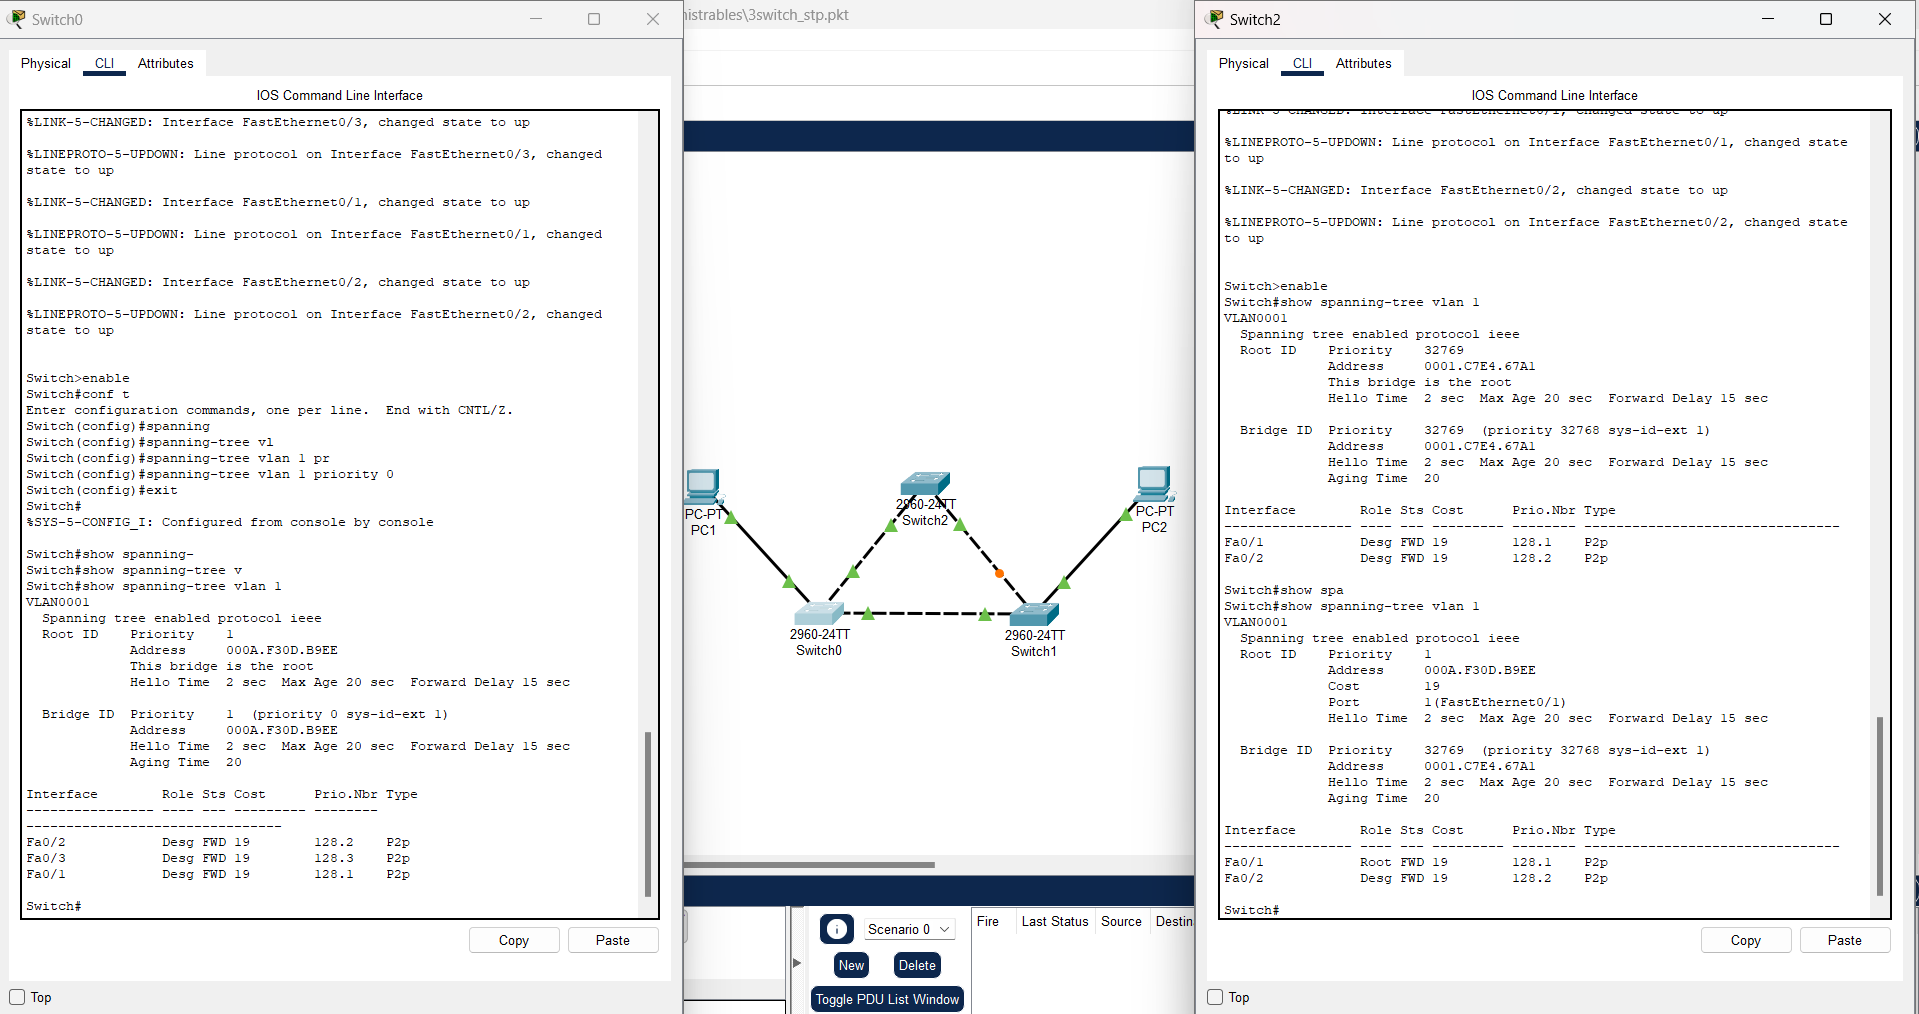
\includegraphics[width=0.825\linewidth]{img_10} 
        \linebreak
        \small {\bfseries Figura 9}: Forzado de elección root Switch0 con priority 0.
    \end{center}

    \subsection{Tormenta de broadcast}
    Al desactivar el protocolo STP en todos los switches se elimina el control de redundancias, lo que al realizar el testeo de un simple PDU de PC1 a PC2 desata una tormenta interminable de paquetes rebotan de un lado hacia el otro llenando el ancho de red. Esto y las configuraciones realizadas se pueden apreciar en las imágenes de Figura 10 y 11.
    \begin{center}
        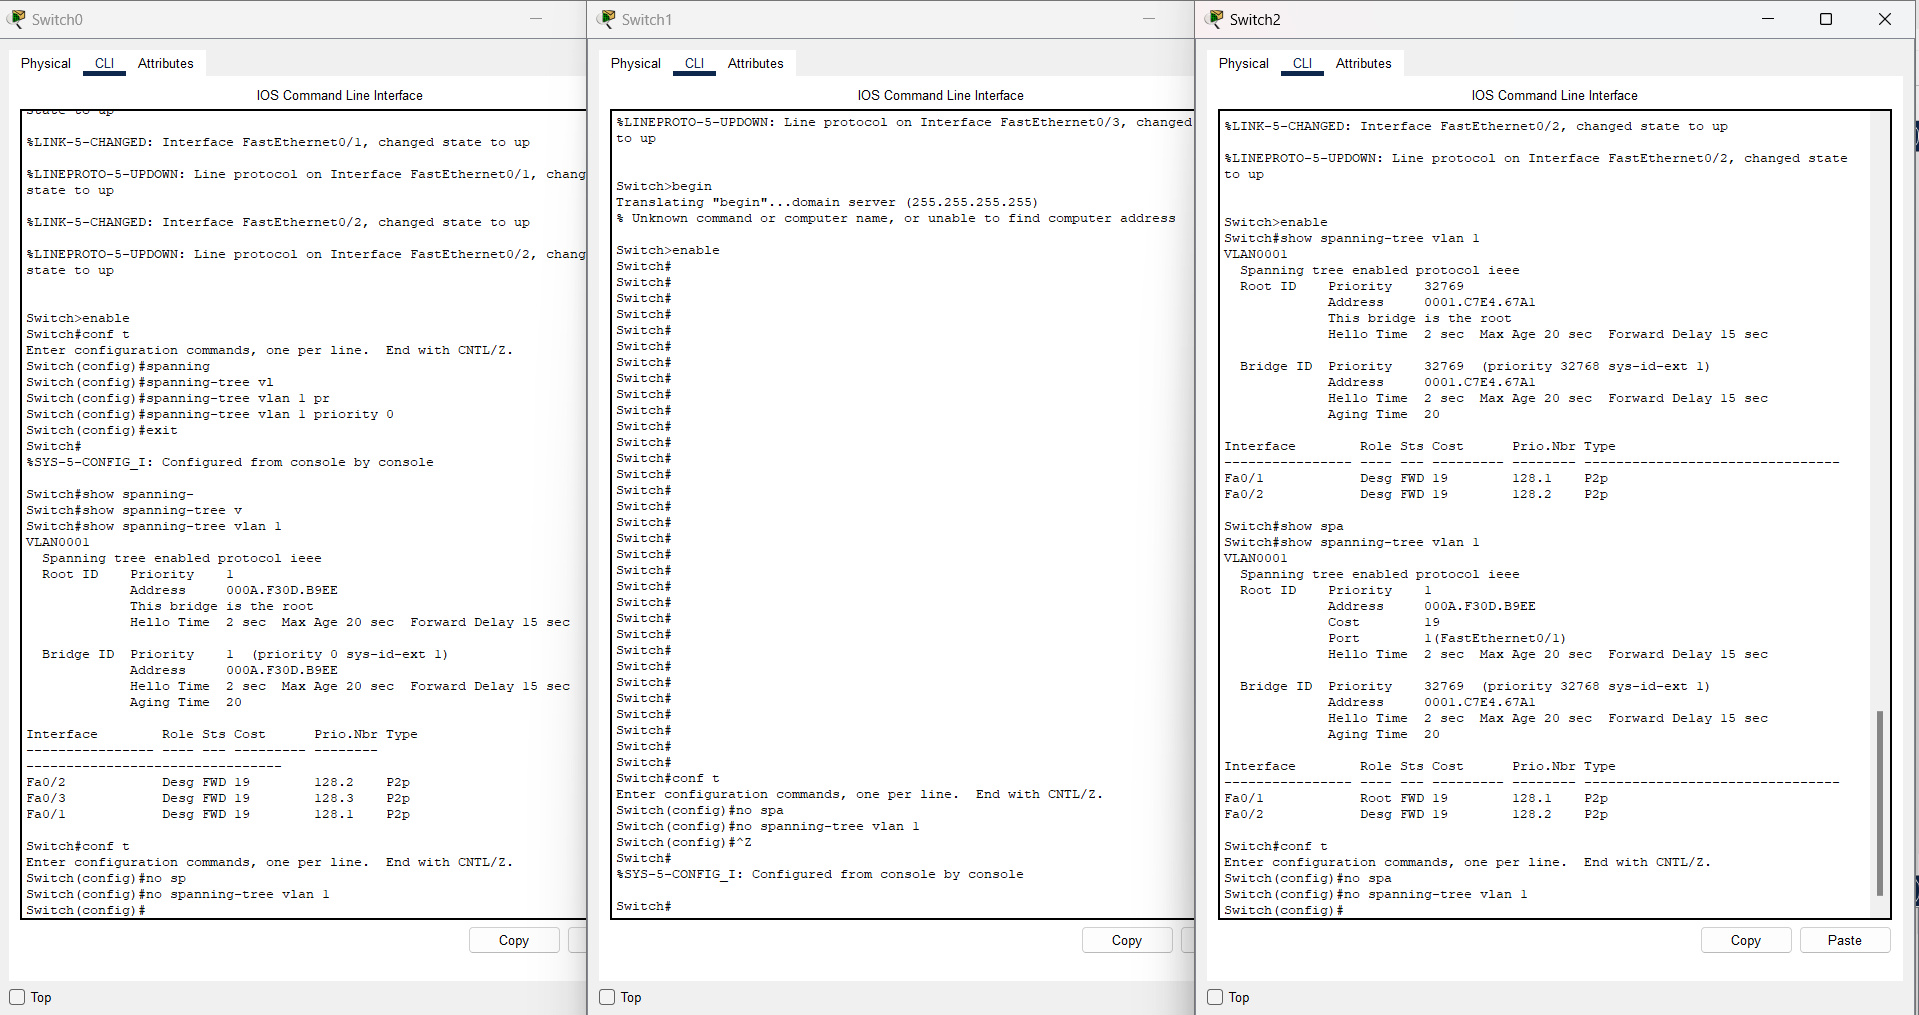
\includegraphics[width=0.875\linewidth]{img_11} 
        \linebreak
        \small {\bfseries Figura 10}: Configuración de desactivación protocolo STP en switches 1, 2 y 3.
    \end{center}

    \begin{center}
        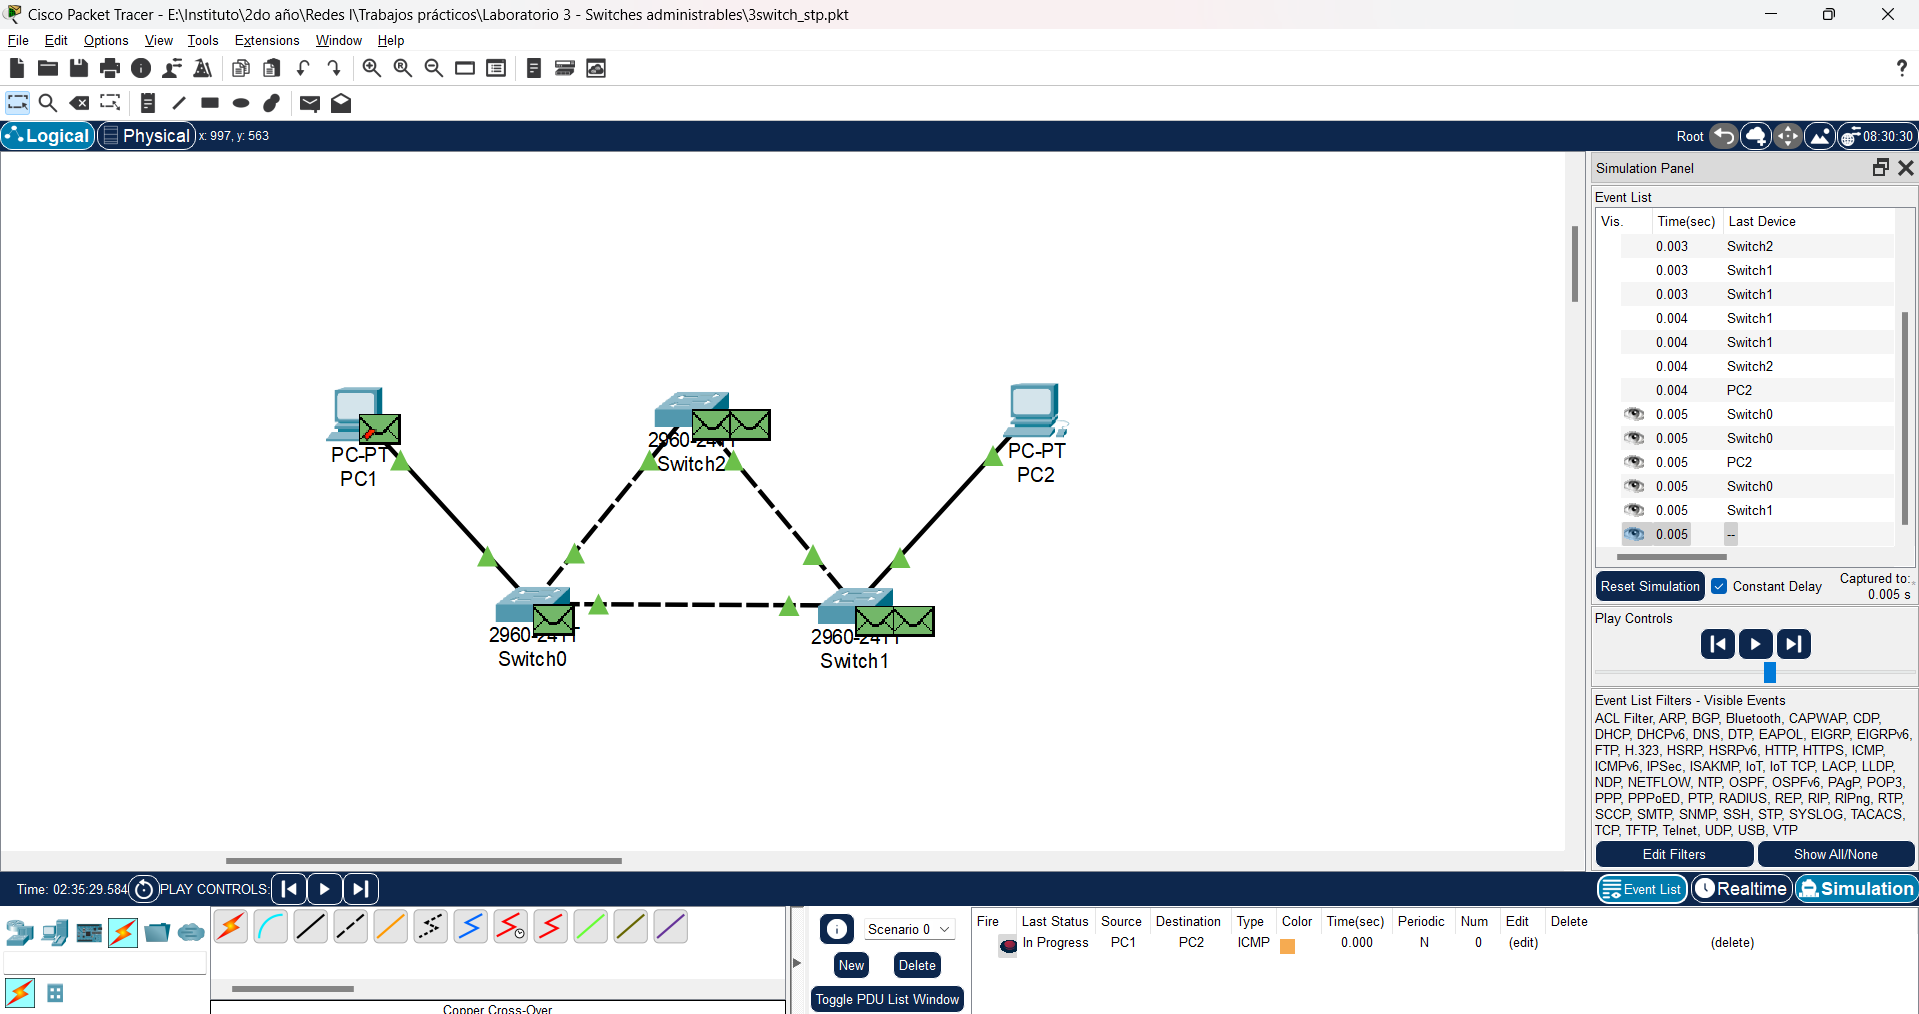
\includegraphics[width=0.475\linewidth]{img_13} 
        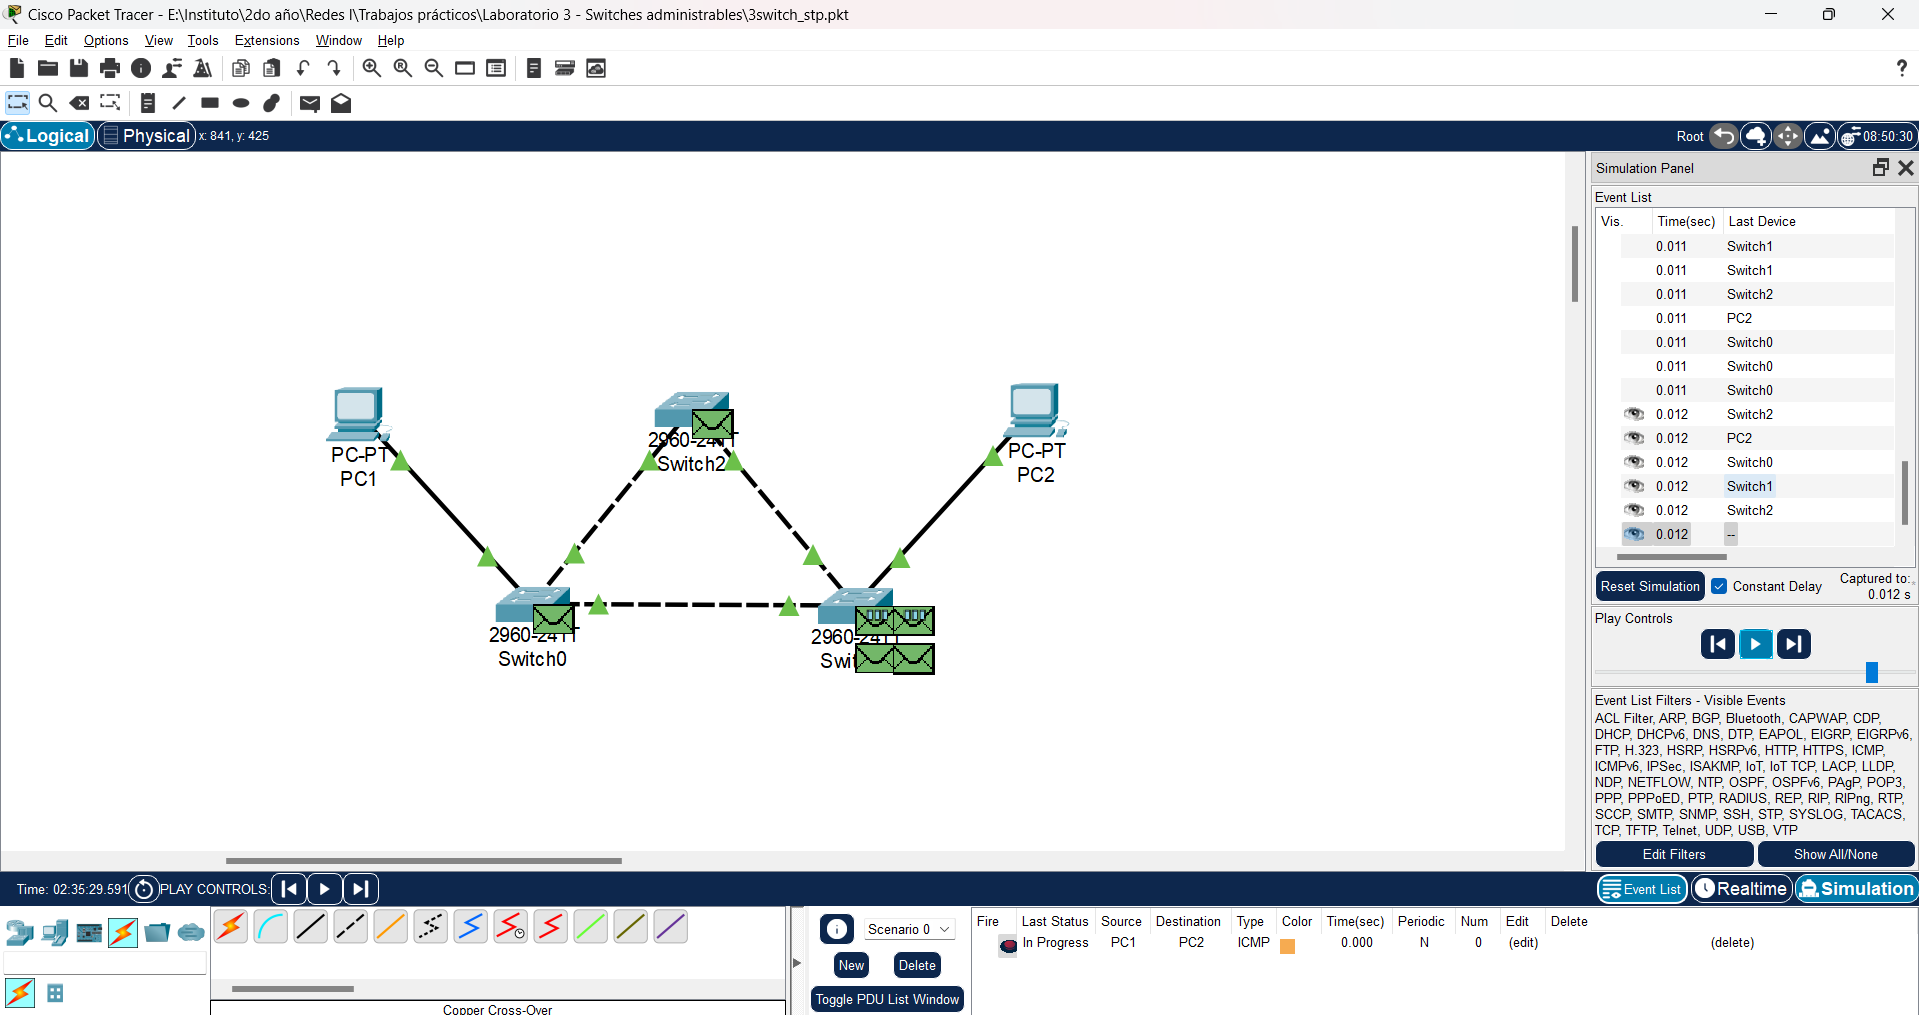
\includegraphics[width=0.475\linewidth]{img_14} 
        \linebreak
        \small {\bfseries Figura 11}: Tormenta de broadcast debido a la falta de protocolo STP.
    \end{center}

    La red se encuentra tan saturada debido a la tormenta de paquetes que viajan de un lado hacia el otro, que al intentar realizar un simple ping de PC1 a PC2, este no se puede completar debido a la congestión.

    \begin{center}
        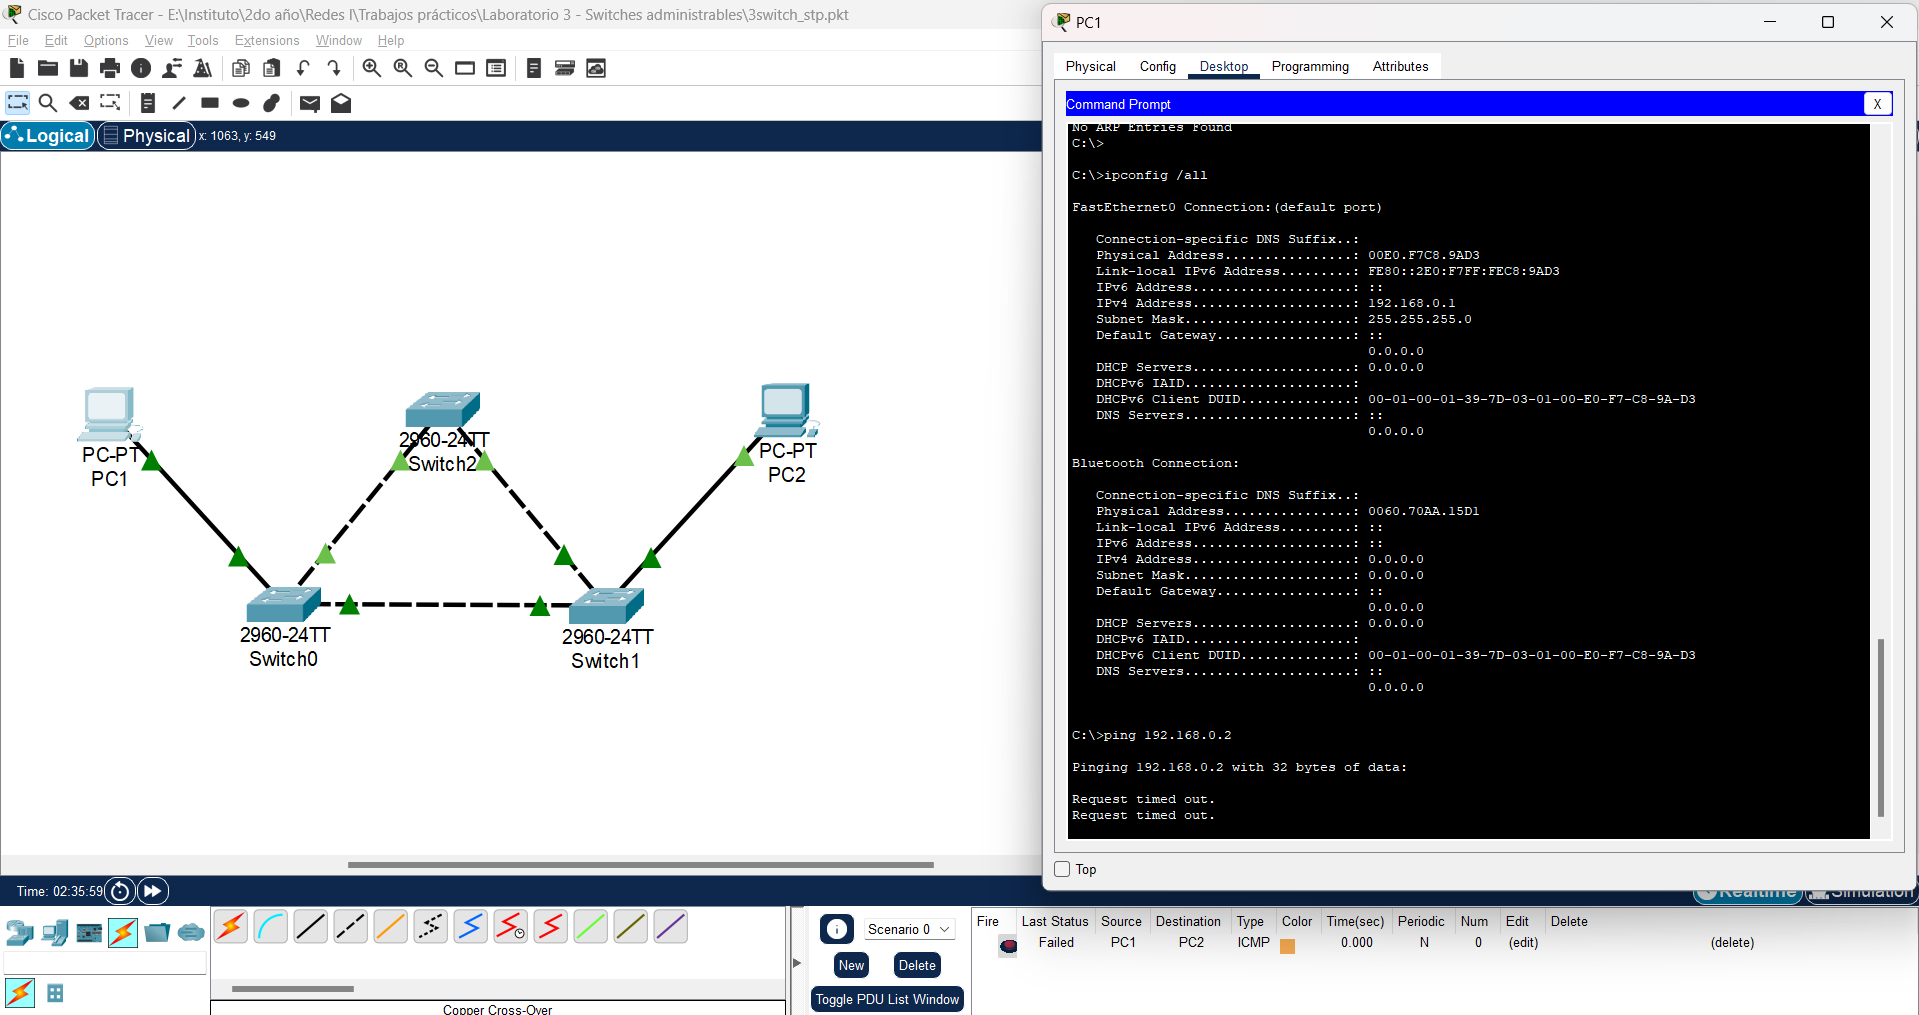
\includegraphics[width=0.875\linewidth]{img_15} 
        \linebreak
        \small {\bfseries Figura 12}: ping en timeout debido a congestión de red.
    \end{center}

    \pagebreak

    \section{Virtual LANs}
    Al realizar la configuración del escenario solicitada y entablar una primera comunicación entre PC11 y PC13, podemos observar que el paquete ARP viaja al router y se propaga por el resto de los dispositivos, tal como lo indica en el pdf del enunciado, todos los dispositivos se encuentran en la misma órbita.

    \begin{center}
        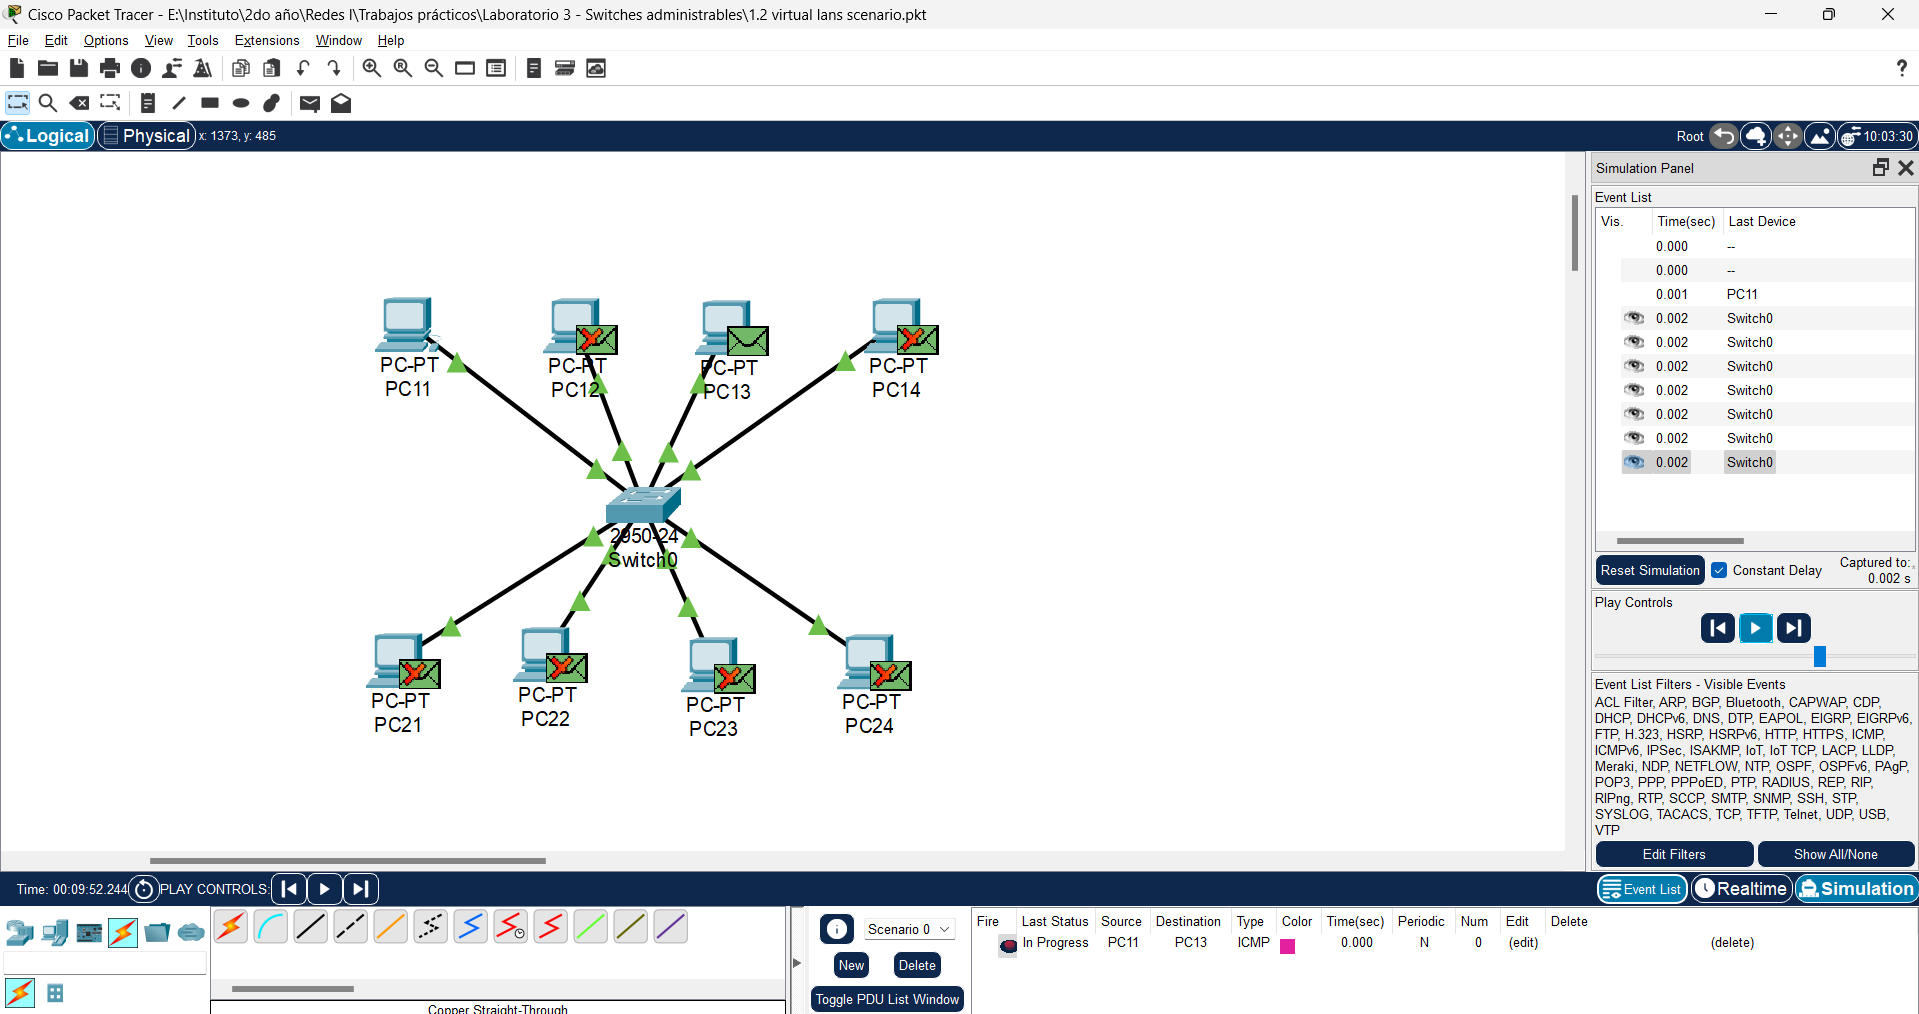
\includegraphics[width=0.775\linewidth]{img_17}  
        \linebreak
        \small {\bfseries Figura 13}: paquete ARP antes de separar los dispositivos en 2 VLANs.
    \end{center}

    Una vez configuradas las VLANs y habiendo separado de PC11 a PC14 en la VLAN2, y de PC21 a PC24 en la VLAN3 utilizando los comandos {\bfseries switchport} (comando que permite configurar los modos de operación, VLAN permitida, prioridad de tráfico, entre otras, de uno o un grupo de puertos de un switch).\\
    El paquete ARP enviado en broadcast al switch ahora únicamente se envía a los dispositivos en la misma VLAN de la que se realizó la solicitud. En este caso enviamos un simple PDU de PC11 a PC14 (previamente se limpió la tabla ARP de PC11 con el comando {\bfseries arp -d}) y como se puede apreciar en la figura 14, se realiza el ARP boardcast de manera correcta dentro de VLAN 2.

    \begin{center}
        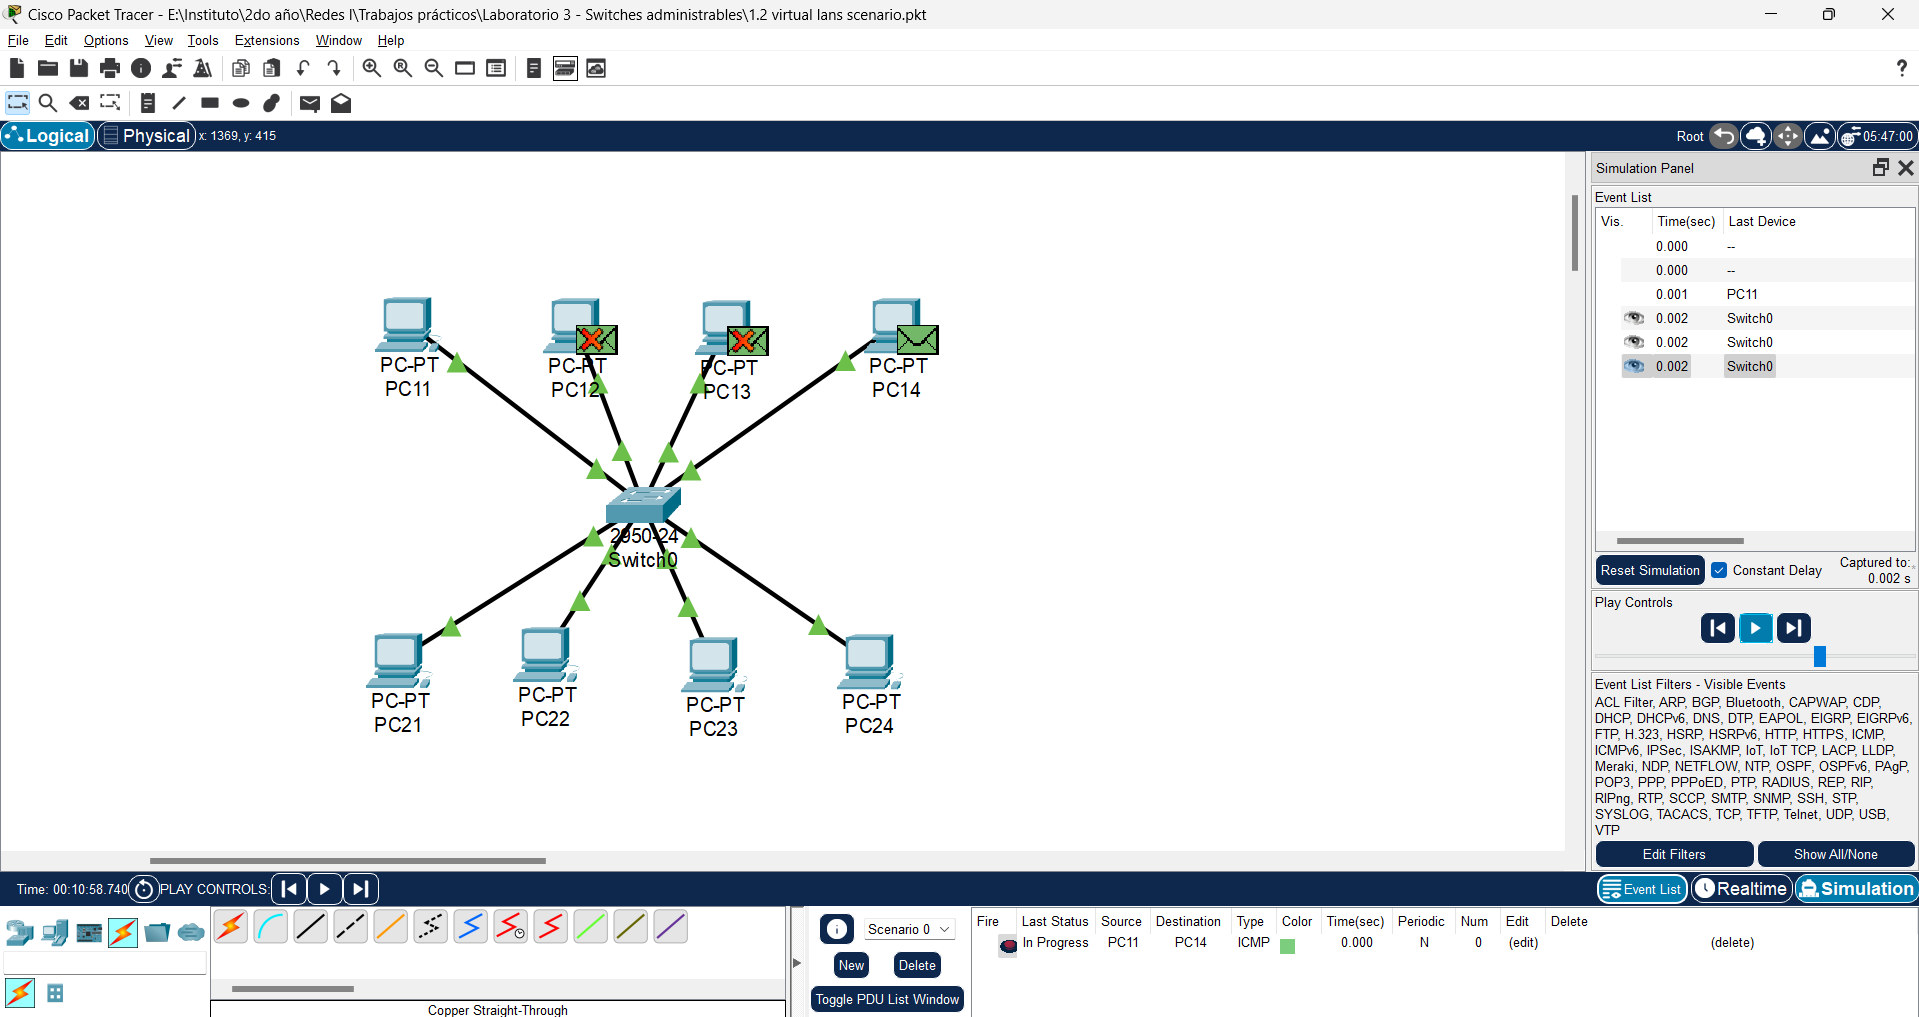
\includegraphics[width=0.775\linewidth]{img_18}  
        \linebreak
        \small {\bfseries Figura 14}: conexión correcta entre dispositivos en una misma VLAN.
    \end{center}

    \pagebreak

    \subsection{VLAN con más de un switch}
    Realizado el cambio en la topología para que la el escenario sea idéntico al de la Figura4 del enunciado, se puede comprobar que la comunicación entre PC11 en VLAN 2 del Switch1 puede comunicarse correctamente con PC14 en VLAN 2 del Switch2. El paquete ARP enviado desde PC11 a PC14 fué enviado al Switch1, éste lo envió a PC12 y a Switch2, y posteriormente Switch2 lo envió a PC13 y PC14 realizando el camino correcto y recibiendo la respuesta correctamente para que PC11 pueda ahora enviar el PDU a su destino.

    \begin{center}
        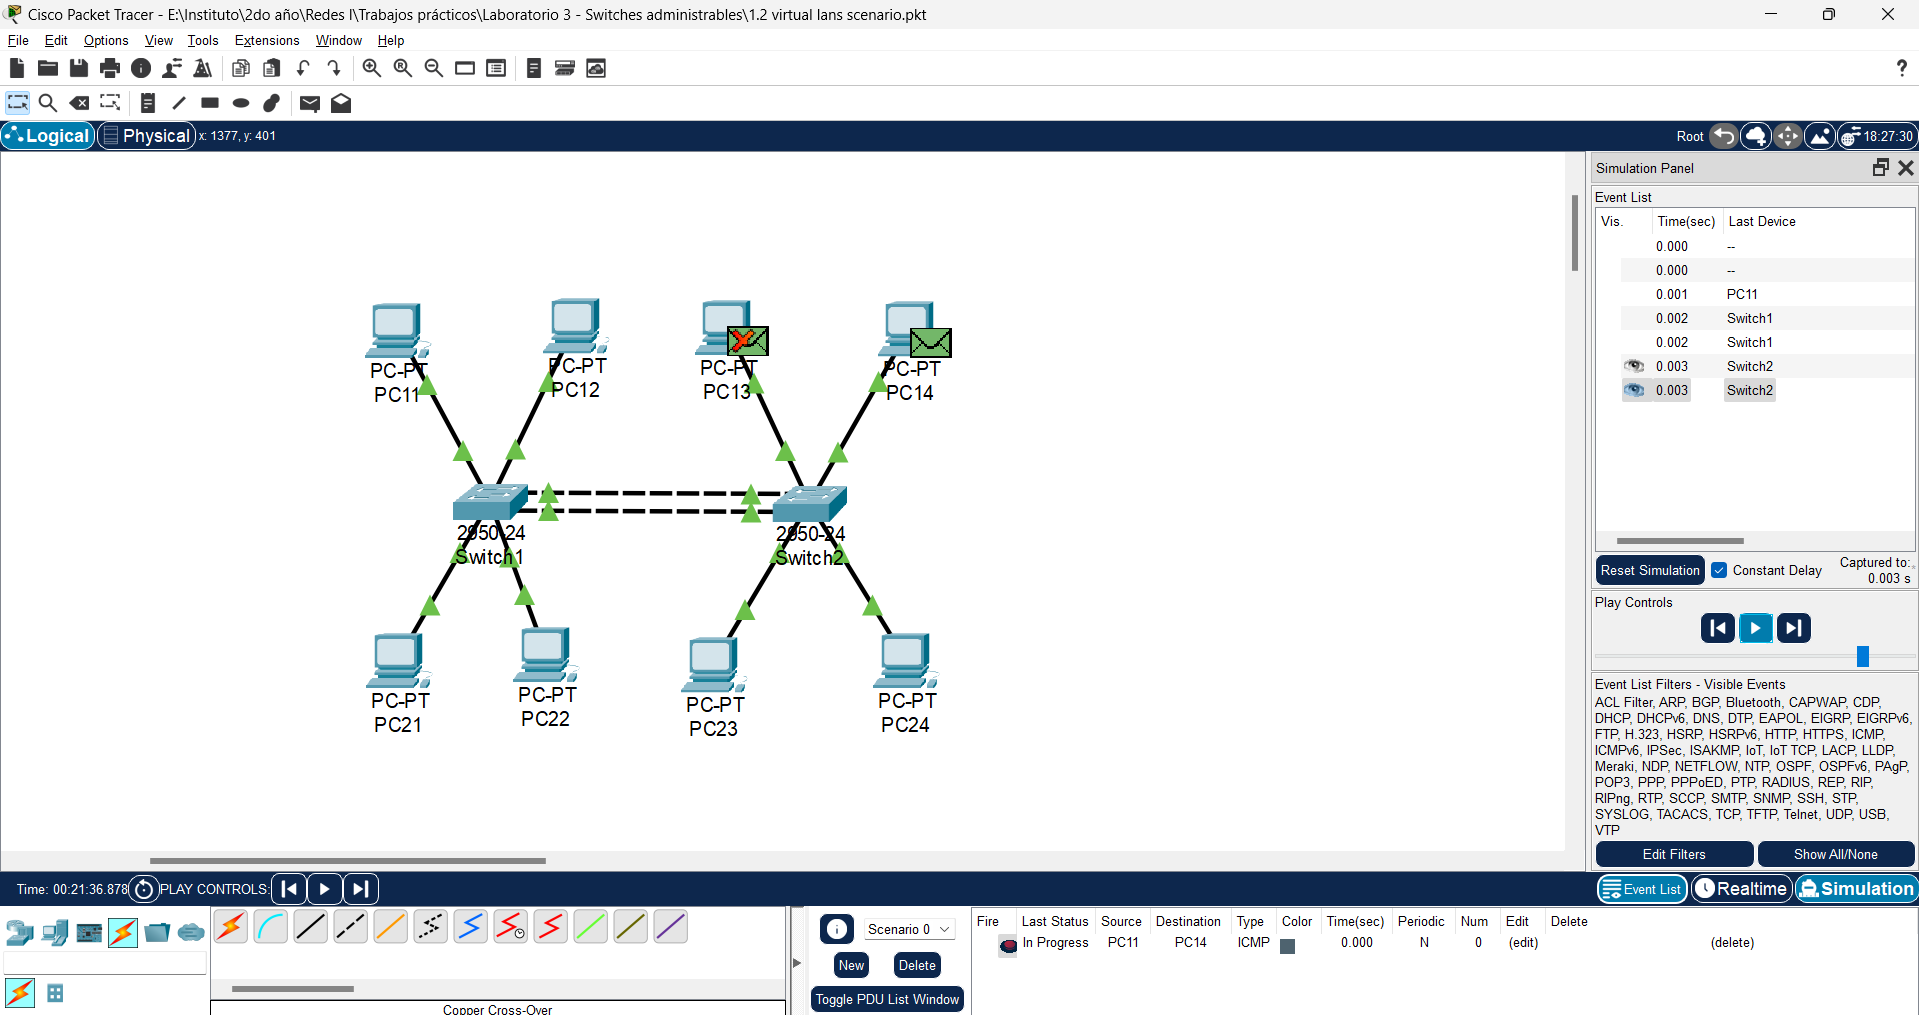
\includegraphics[width=0.775\linewidth]{img_19}  
        \linebreak
        \small {\bfseries Figura 15}: comunicación entre PC11 y PC14 en diferentes switches pero en misma VLAN, con switches interconectados en puertos de misma VLAN.
    \end{center}

    \subsection{Port trucking}
    Para realizar el trabajo de esta sección, se debió actualizar los switches 2950-24 por dos switches 2960-24TT debido a que los 2950, no contaban con el puerto Gigabit Ethernet.\\
    Valores encontrados con comando {\bfseries show interface gigabitEthernet 0/1 switchport}:

    \begin{center}
        \begin{tabular}{| p{4cm} | p{3cm} | p{11cm} |}\hline
            {\bfseries Variables} & {\bfseries Valor} & {\bfseries Descripción} \\\hline
            Administrative Mode & dynamic auto & Muestra el modo de administración configurado. \\\hline
            Operational Mode & static access & Muestra el modo de operación configurado. \\\hline
            Administrative Trunking Encapsulation & dotlq & Muestra el método de encapsulación administrativa. \\\hline
            Trunking VLANs Enabled & All & Muestra la lista de VLANs habilitadas del la línea de gestión de múltiples señales (troncal/trunk). \\\hline
        \end{tabular}
    \end{center}

    \begin{center}
        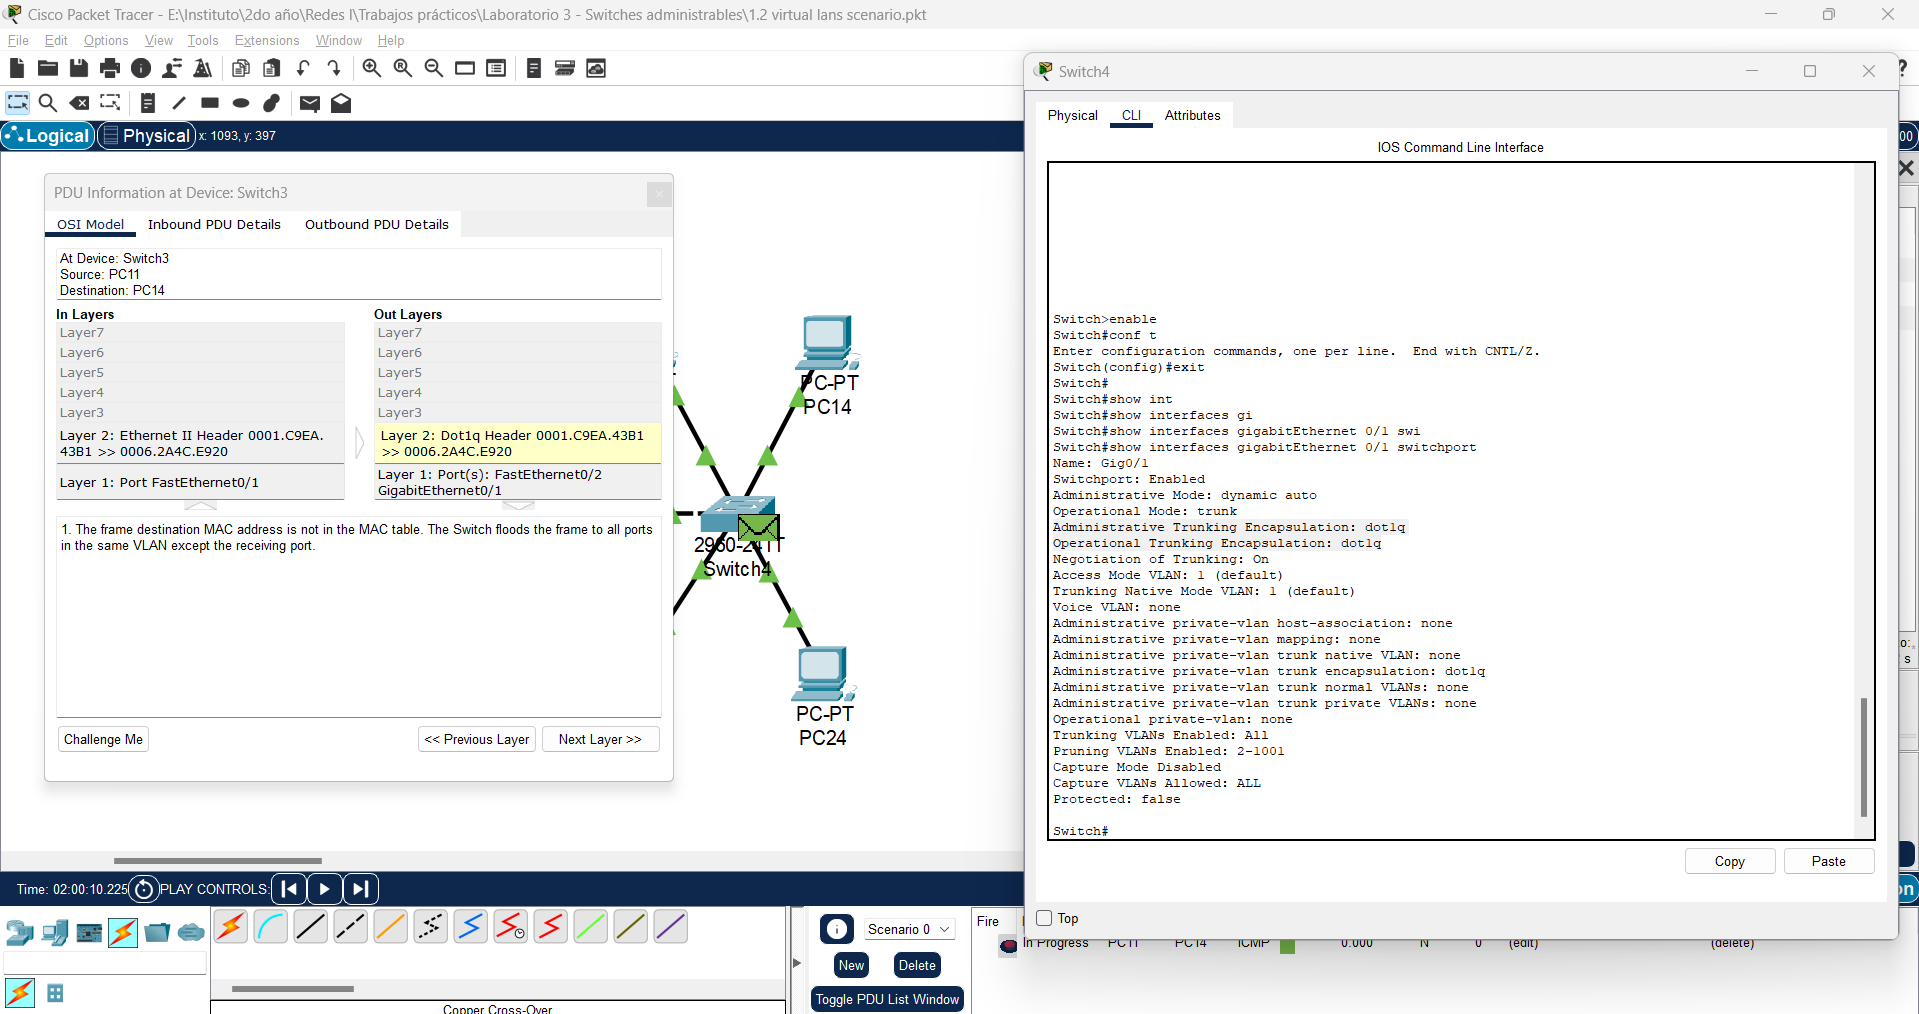
\includegraphics[width=0.775\linewidth]{img_20}  
        \linebreak
        \small {\bfseries Figura 16}: encapsulamiento de PDU con el valor dotlq de la configuración de la interfaz demostrada en la tabla 2.2.
    \end{center}

    {\bfseries Filtro de tráfico}: para filtrar el tráfico por tags, utilicé la documentación del switch catalyst2960 (indicado en las referencias). El primer paso es eliminar todas las vlan permitidas (ya que por defecto Trucking VLAN viene configurada como All), para esto utilicé el comando {\bfseries switchport trunk allowed vlan none} en la configuración de la interfaz {\bfseries gigabitEthernet 0/1}. Luego habilité como primer entrada que se permitiera el tráfico de la VLAN 2 con el comando {\bfseries switchport trunk allowed vlan add 2}. Esto filtrará TODO el tráfico excepto el de VLAN 2.\\
    En la simulación se enviaron dos PDU, uno de PC11 a PC13 (ambas pertenecen a VLAN 2, y donde el PDU debería viajar encapsulado por el troncal entre switches), y otro de PC21 a PC23 (ambas pertenecen a VLAN 3, y donde ese paquete debería viajar por el troncal entre switches). Con la configuración realizada podemos corroborar que el paquete de PC11 llegó a destino correctamente, pero el de PC21 no debido al filtro realizado.\\

    \begin{center}
        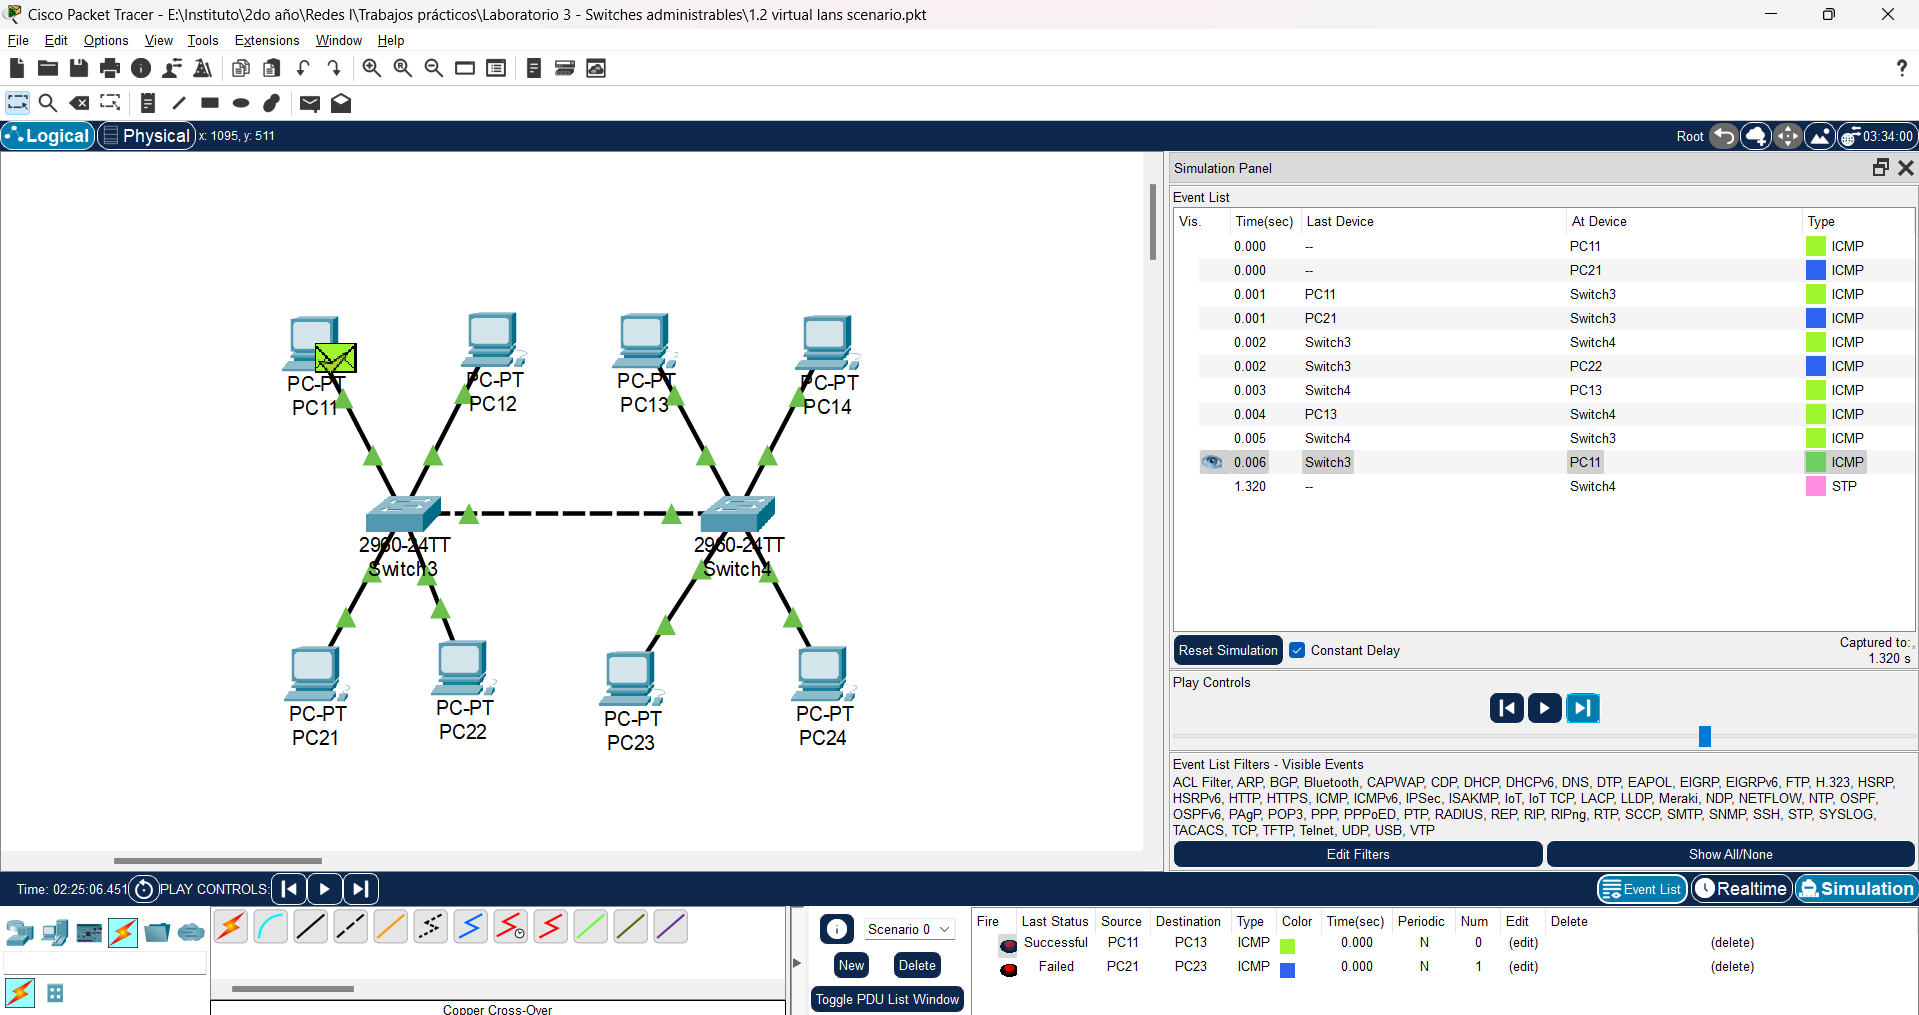
\includegraphics[width=0.775\linewidth]{img_21}  
        \linebreak
        \small {\bfseries Figura 17}: Filtro tráfico VLAN.
    \end{center}

    \pagebreak
    \section{Port aggregation}
    El Port Aggregation Protocol es un protocolo de cisco, utilizado para la tecnología EtherChannel. Consiste en agrupar varios puertos FastEthernet o GigabitEthernet, entre 2 switches en un único canal lógico.\\
    \begin{itemize}
        \item No es necesario actualizar el enlace a una conexión más rápida y mas costosa para tener mayor ancho de banda.
        \item Se cuenta con un balanceo de carga entre los enlaces que forman parte.
        \item Se crea una agregación que se ve como un único canal lógico.
        \item EtherChannel proporciona redundancia.
    \end{itemize}

    Cuando se habilita, PAgP también administra el EtherChannel. Los paquetes PAgP se envían cada 30 segundos. PAgP tiene varios modos:

    \begin{itemize}
        \item On (encendido): miembro del canal sin negociación (sin protocolo). Este modo obliga a la interfaz a proporcionar un canal sin PAgP.
        \item Deseado: pregunta activamente, si el otro lado puede participar va a hacerlo. Este modo coloca una interfaz en un estado de negociación activa en el que inicia negociaciones con otras interfaces al enviar paquetes PAgP.
        \item Automático: espera pasivamente al otro lado. Coloca una interfaz en estado de negociación pasiva, en el que la interfaz responde a los paquetes PAgP que recibe, pero no inicia negociaciones.
    \end{itemize}

    \begin{center}
        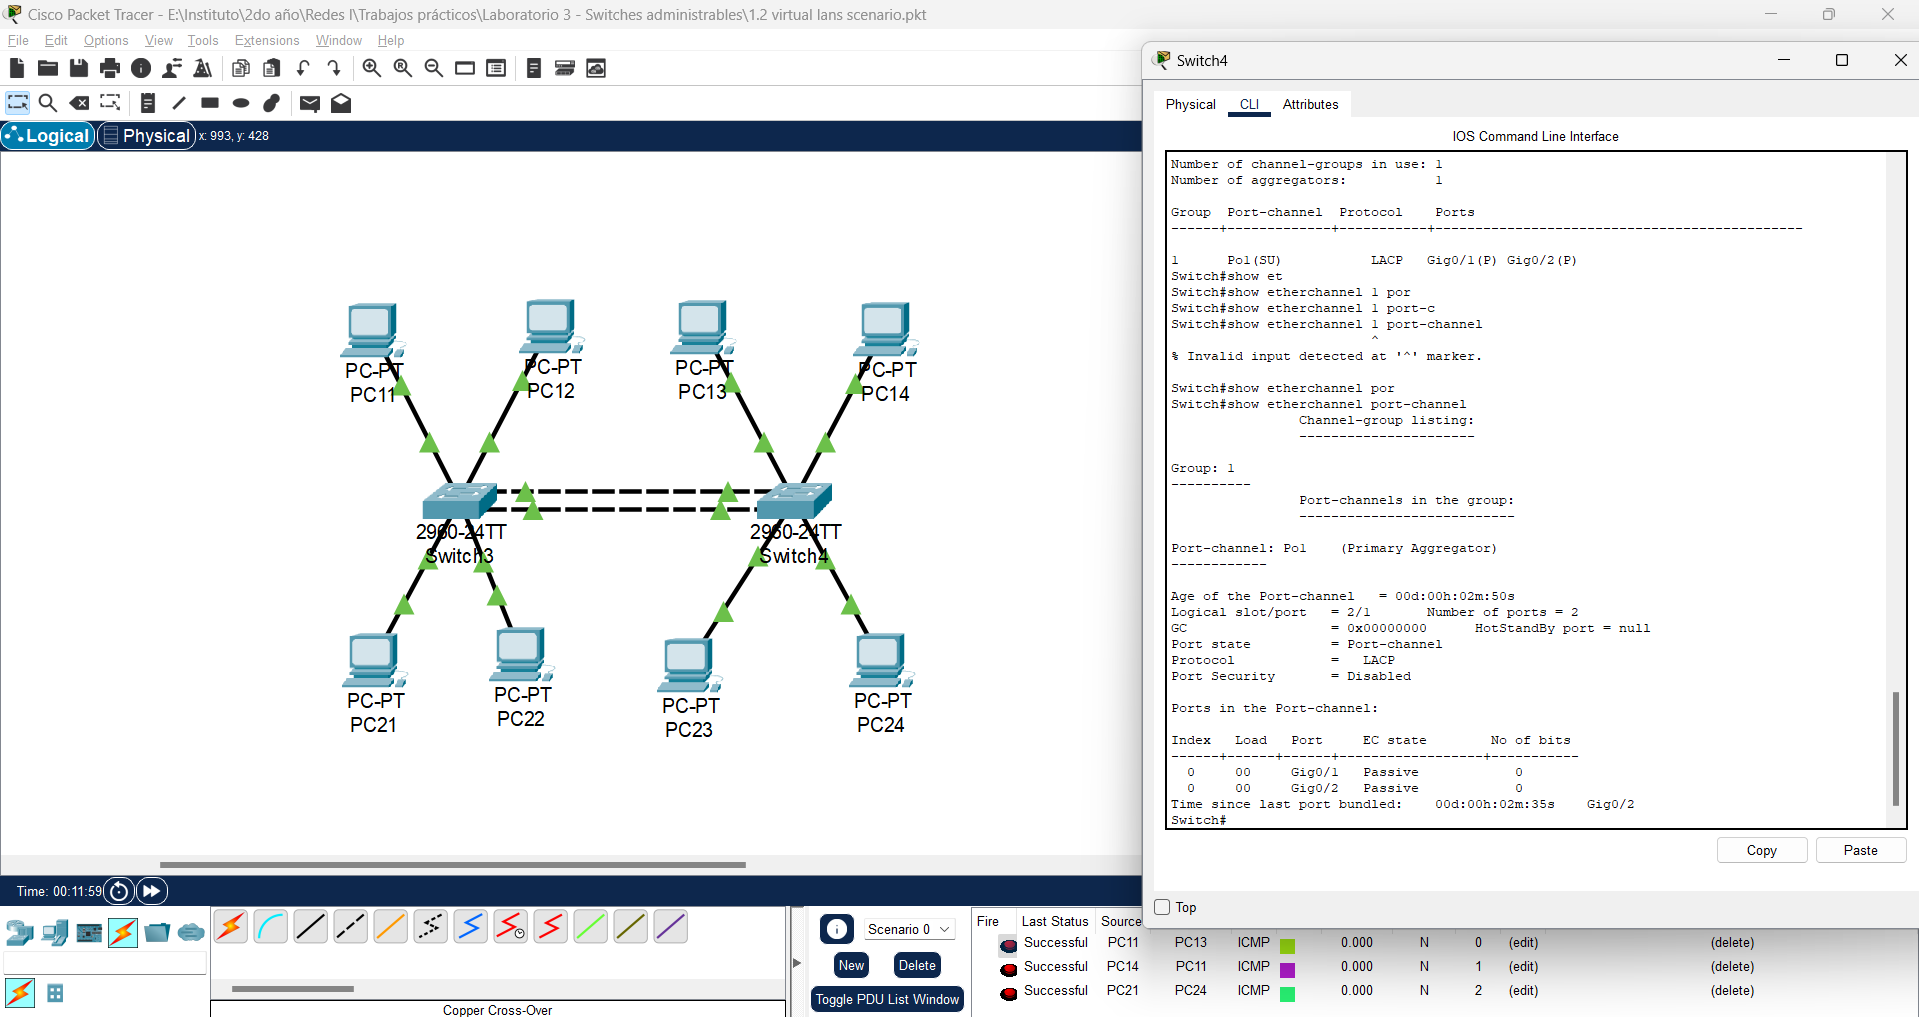
\includegraphics[width=0.775\linewidth]{img_22}  
        \linebreak
        \small {\bfseries Figura 18}: Configuración final del escenario de red.
    \end{center}


    \pagebreak
    \section{Referencias}
        \begin{itemize}
            \item \href{https://github.com/MarianC312/Laboratorio_3_Switches_Administrables}{Repositorio GitHub}
            \item \href{https://www.cisco.com/c/en/us/td/docs/switches/lan/catalyst2960/software/release/12-2_25_see/command/reference/cr.pdf}{Documentación Switch Cisco Catalyst 2960}
            \begin{itemize}
                \item Cap. 2 - Pag. 332-333: Table 2-22 show interfaces switchport Field Descriptions
                \item Cap. 2 - Pag. 535-536: switchport trunk 
            \end{itemize}
            \item \href{https://ccnadesdecero.es/agregacion-de-enlaces-pagp-lacp/}{Protocolos PAgP y LAPC}
        \end{itemize}
\end{document}